\section{Architectural Design} \label{sec architectural design}

\subsection{Overview}

The PowerEnJoy's software architecture will be described starting from an high level view up to an in detail view of a specific system component. Going into details will be discussed the roles of these components and how can they interact through several interfaces.

A static and dynamic viewpoint are provided in order to better explaining how the architecture works through its components.

\subsection{High Level View}

In order to explain the role of the system's components, it's better considering the layers involved for each component.
There are 3 different distinguishable layers:

\begin{description}
	\item[{\color{green} Presentation}:] this layer provides a data processing for a GUI and/or a GUI itself.
	\item[{\color{blue} Application}:] this layer provides one or more logic functionalities. Functionalities could be core, if they are performing an essential function for the system, or peripheral, if they are managing interactions between core functionalities or interfaces between system's components.
	\item[{\color{red} Data}:] this layer provides a way to store and retrieve the essential data for the system.
\end{description}
The main components of the system are the following:

\begin{description}
	\item[Database:] a data layer that supports a RDBMS.
	\item[Application server:] an application layer responsible for the whole application logic of the system. All the policies, the algorithms and the computation are performed here. This layer offers a service-oriented interface.
	\item[Web server:] a presentation layer responsible for translating HTTPS requests into API requests and API responses into HTTPS responses. 
	\item[Mobile application:] a presentation layer directly connected to the application server.
	\item[Car applications:] Cambiarea presentation and application layer that provide utilities to the user and an interface to the server in order to manage the car.
	\item[User's browser:] a presentation layer consisting in a web browser. Not under control of the system.
\end{description}
The following figure shows all the components of the system, highlighting the logic layers for each component, grouped by the physical tiers.

\begin{figure}[H]
	\centering
	\includegraphics[width=\textwidth, keepaspectratio]{diagrams/Tiers.png}
	\caption{High level view of the PowerEnJoy architecture.}
	\label {fig:tiers}
\end{figure}

\subsection{Component View}

\subsubsection{Database}

The server database of the system runs MySQL Community Edition 5.7 with InnoDB as default storage engine. InnoDB provides the standard ACID-compliant transaction features.

The database is only and directly connected to the application server through the standard network interface, described in \autoref{sec:component-interfaces}.

The following properties are satisfied:
\begin{itemize}
	\item users' passwords are not saved in plain-text, but they are salted with 8 random bytes, added to the password, and encrypted using the SHA-1 algorithm. The 8 random bytes are different for each password and obviously stored.
	\item access to the data must be granted only to authorized users possessing the right credentials.
	\item every software component that needs to access the DBMS must do so with the minimum level of privilege needed to perform the operations.
\end{itemize}
All the persistent application data is stored in the database. The relational model is illustrated in the following figure.

\begin{figure}[H]
	\centering
	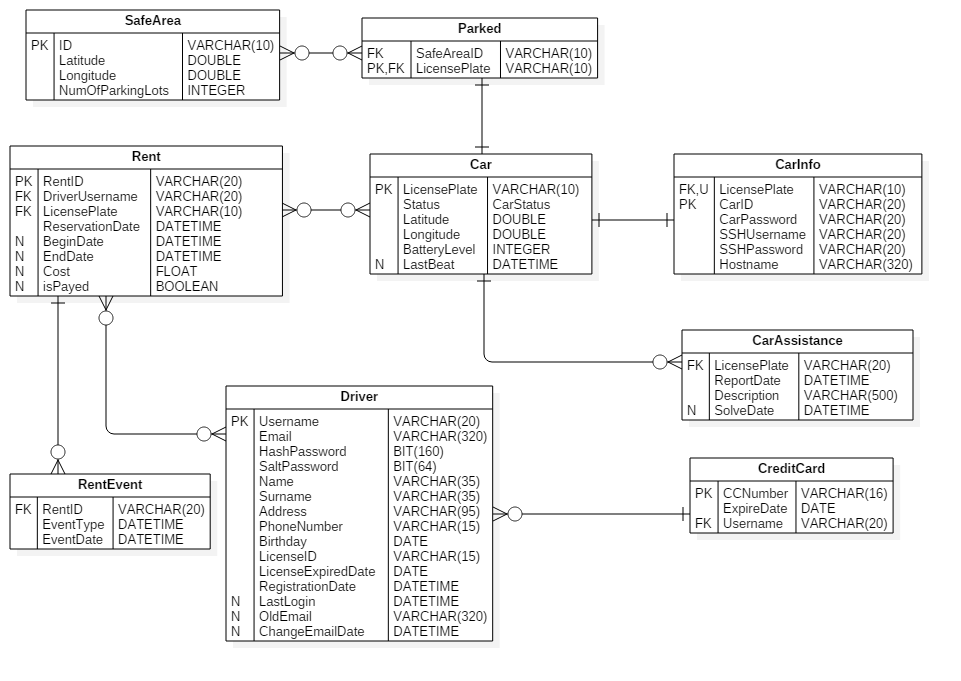
\includegraphics[width=\textwidth, keepaspectratio]{diagrams/Relational.png}
	\caption{Relational model of the database schema.}
	\label {fig:relational}
\end{figure}

Several triggers are implemented to manage some exceptions. For instance:
\begin{itemize}
	\item the registration is cancelled if a driver has never logged into the system for 10 days since his/her registration.
	\item the rent is aborted if a driver doesn't unlock the reserved car within 1 hour. Cost of the rent is setted to 1 euro.
	\item a report of assistance to a car is generated if it have been passed more than 10 minutes from the last car heartbeat.
\end{itemize}

\subsubsection{Application Server}

The application servers are implemented using Java EE; they runs on GlassFish server.

The business logic is implemented by custom-built EJB. Cosa sono e come sono formati. Given that the state of users, cars and rents is stored in the database, all the EJB are stateless.

Parlare delle servlet

The access to the DBMS is not implemented with direct SQL queries: instead, it is completely wrapped by the JPA. The object-relation mapping is done by entity beans. They are simple java classes without a constructor and fulfilled by getter and setter methods for each attributes, that correspond to fields of a database table. EJBs use those entity beans in order to read and write on the database.

FARE CLASSI UML

Session Beans used for the application server are shown in~\autoref{fig:session-beans}.

\subsubsubsection{DriverManager}
This bean manages all the driver management features: user registration, user deletion, user profile editing.
User registration provides a function that sends an email, with a password and some guidelines, after the registration.

\subsubsubsection{LogbookManager}
This bean allows users to fetch the history of their past rents.

\subsubsubsection{ReservationManager}
This bean allows users to get information about the available cars and reserve cars.

\subsubsubsection{DriverRentManager}
This bean allows users to unlock a reserved cars and fetch information about the current rents.

\subsubsubsection{CarHeartBeat}
This bean manages information coming from cars. It also provides a function responsible for closing cars.

\subsubsubsection{CarRentManager}
This bean manages rental features: current rental charge, nearby safe areas.

\begin{figure}[H]
	\centering
	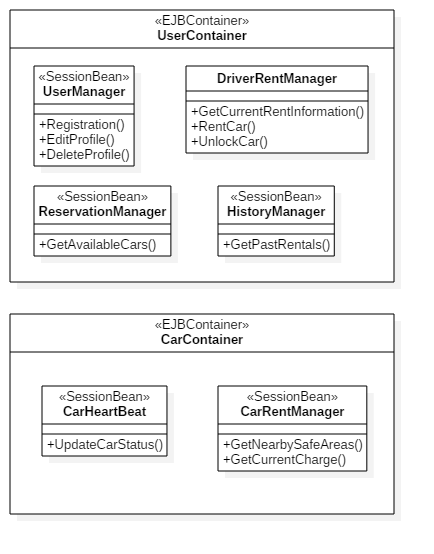
\includegraphics[width=\textwidth, keepaspectratio]{diagrams/SEJBs.png}
	\caption{Session EJBs implemented server side.}
	\label {fig:session-beans}
\end{figure}

\subsubsection{Web Server}

The web server runs on GlassFish server. It's implemented using JSP; java EE web components useful when the goal of the web server is to translate RESTful API requests/responses into  HTTP/HTTPS requests/responses. Thanks to JSPs, developers can focusing better on the GUI.

The API requests are managed by a translator, an internal Java interface that simply the JSP job translating methods calls into API calls.


\begin{figure}[H]
	\centering
	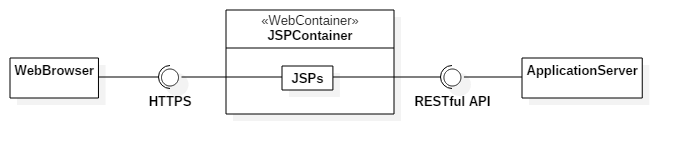
\includegraphics[width=\textwidth, keepaspectratio]{diagrams/WebComponents.png}
	\caption{The components and the interfaces of the web tier.}
	\label {fig:web-components}
\end{figure}

Even if REST is a stateless architectural style, JSPs lead users to a stateful communication saving the session; in order to avoid further insertion of user's credentials.

\subsubsection{Car Applications}

Every car hosts a computer with a linux distribution of Ubuntu 16.10 as operating system. In any OS is installed openssh-server, in order to access to the car remotly, and two applications:
\begin{description}
	\item[HeartBeat:] this application is always running and sends, every 10 seconds, information about the current state of the car and the rent, to the application server through a single API call. The application server will ignore the rental information if the car is not rented.
	\item[CarGUI:] this application is started everytime the car gets unlocked, and closed everytime the car gets locked. It asks, through API calls, for user information, user's current charges and nearby availabe safe areas, in order to display those information on the GUI.
\end{description}

\begin{figure}[H]
	\centering
	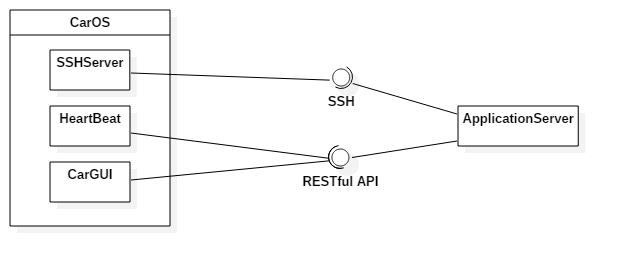
\includegraphics[width=\textwidth, keepaspectratio]{diagrams/CarClientComponents.png}
	\caption{The components and the interfaces of the car client tier.}
	\label {fig:car-client-components}
\end{figure}

\subsubsection{Mobile Application}

The mobile client implementation depends on the specific platform. 
The iOS application is implemented in Swift and mainly uses UIKit framework to manage the UI interface.
Instead, the Android application is implemented in Java and mainly uses android.view package for graphical management.

The application core is composed by a controller which translates the inputs from the UI into remote functions calls via  RESTful APIs. The controller also manages the interaction with the GPS component using  CoreLocation framework in iOS app and LocationListener interface in the Android one.

\begin{figure}[H]
    \centering
    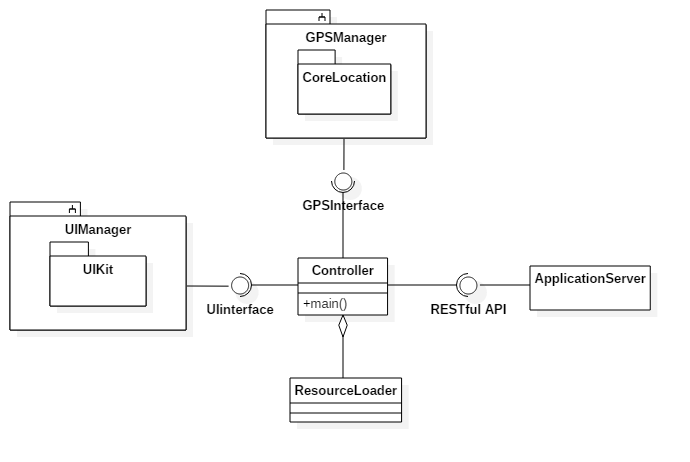
\includegraphics[width=\textwidth, keepaspectratio]{diagrams/iOS.png}
    \caption{The components of the iOS application.}
    \label{fig:ios-app}
\end{figure}

\begin{figure}[H]
    \centering
    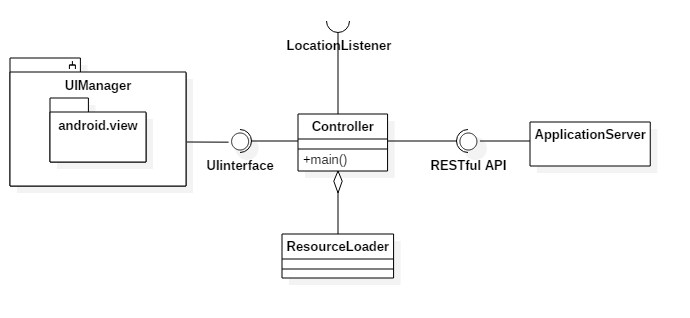
\includegraphics[width=\textwidth, keepaspectratio]{diagrams/Android.png}
    \caption{The components of the Andorid application.}
    \label{fig:android-app}
\end{figure}

\subsection{Component Interfaces}

\subsubsection{Front-ends to Application Server (API)}

As already said, the front-ends applications comunicate with the application server through RESTful API over the HTTPS protocol. They are provided by the application server and use JSON as data representation language.

The detailed RESTful API is described in the following pages. 

Common to all the requests:
\begin{itemize}
	\item the paths must be applied to the application server domain.
	\item a 422 error means that the JSON object has been not created correctly or the values of the objects' fields cannot be processed by the application server. For instance, the username choosen could be already taken or could not match to the regular expression choosen by the system.
	\item requests over HTTP protocol are denied.
\end{itemize}


\subsubsubsection{[User] Creates user}
\begin{figure}[H]
	\noindent
    	\centering
    	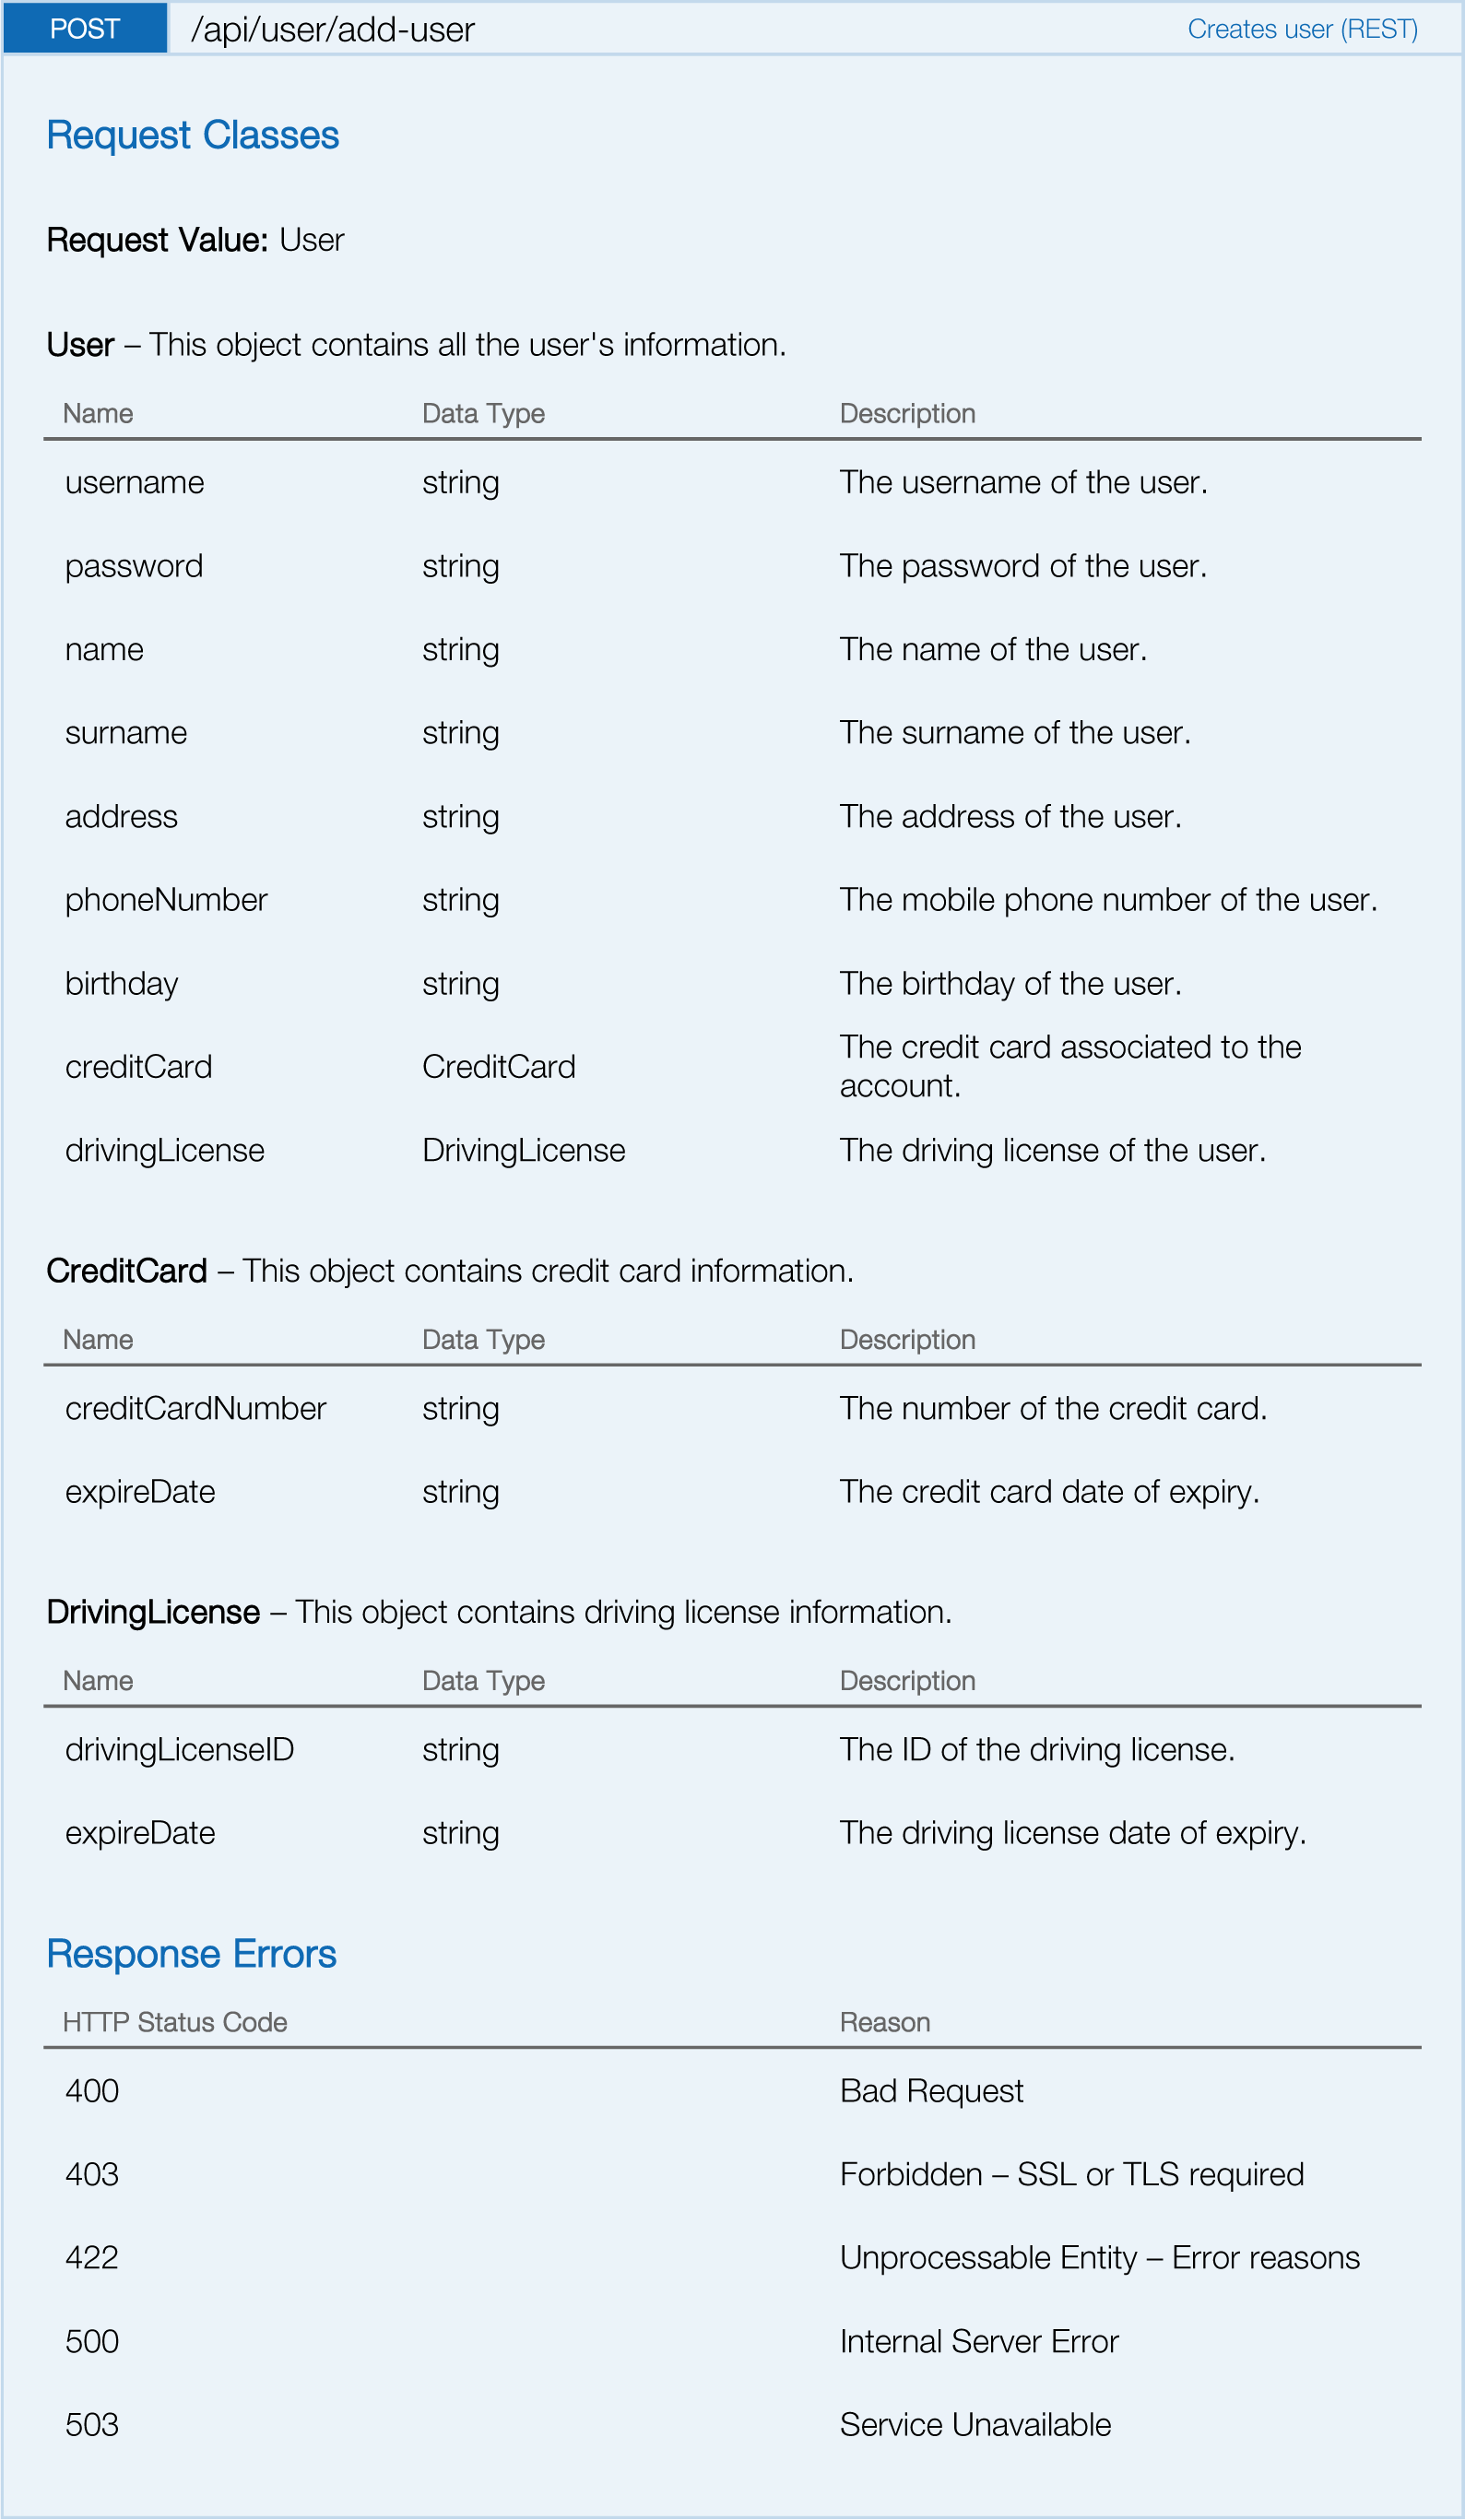
\includegraphics[height=550px, keepaspectratio]{apitables/APIAddUser.png}
    	\label{fig:api-add-user}
\end{figure}

\subsubsubsection{[User] Retrieves user's salt bytes}
\begin{figure}[H]
	\noindent
    	\centering
    	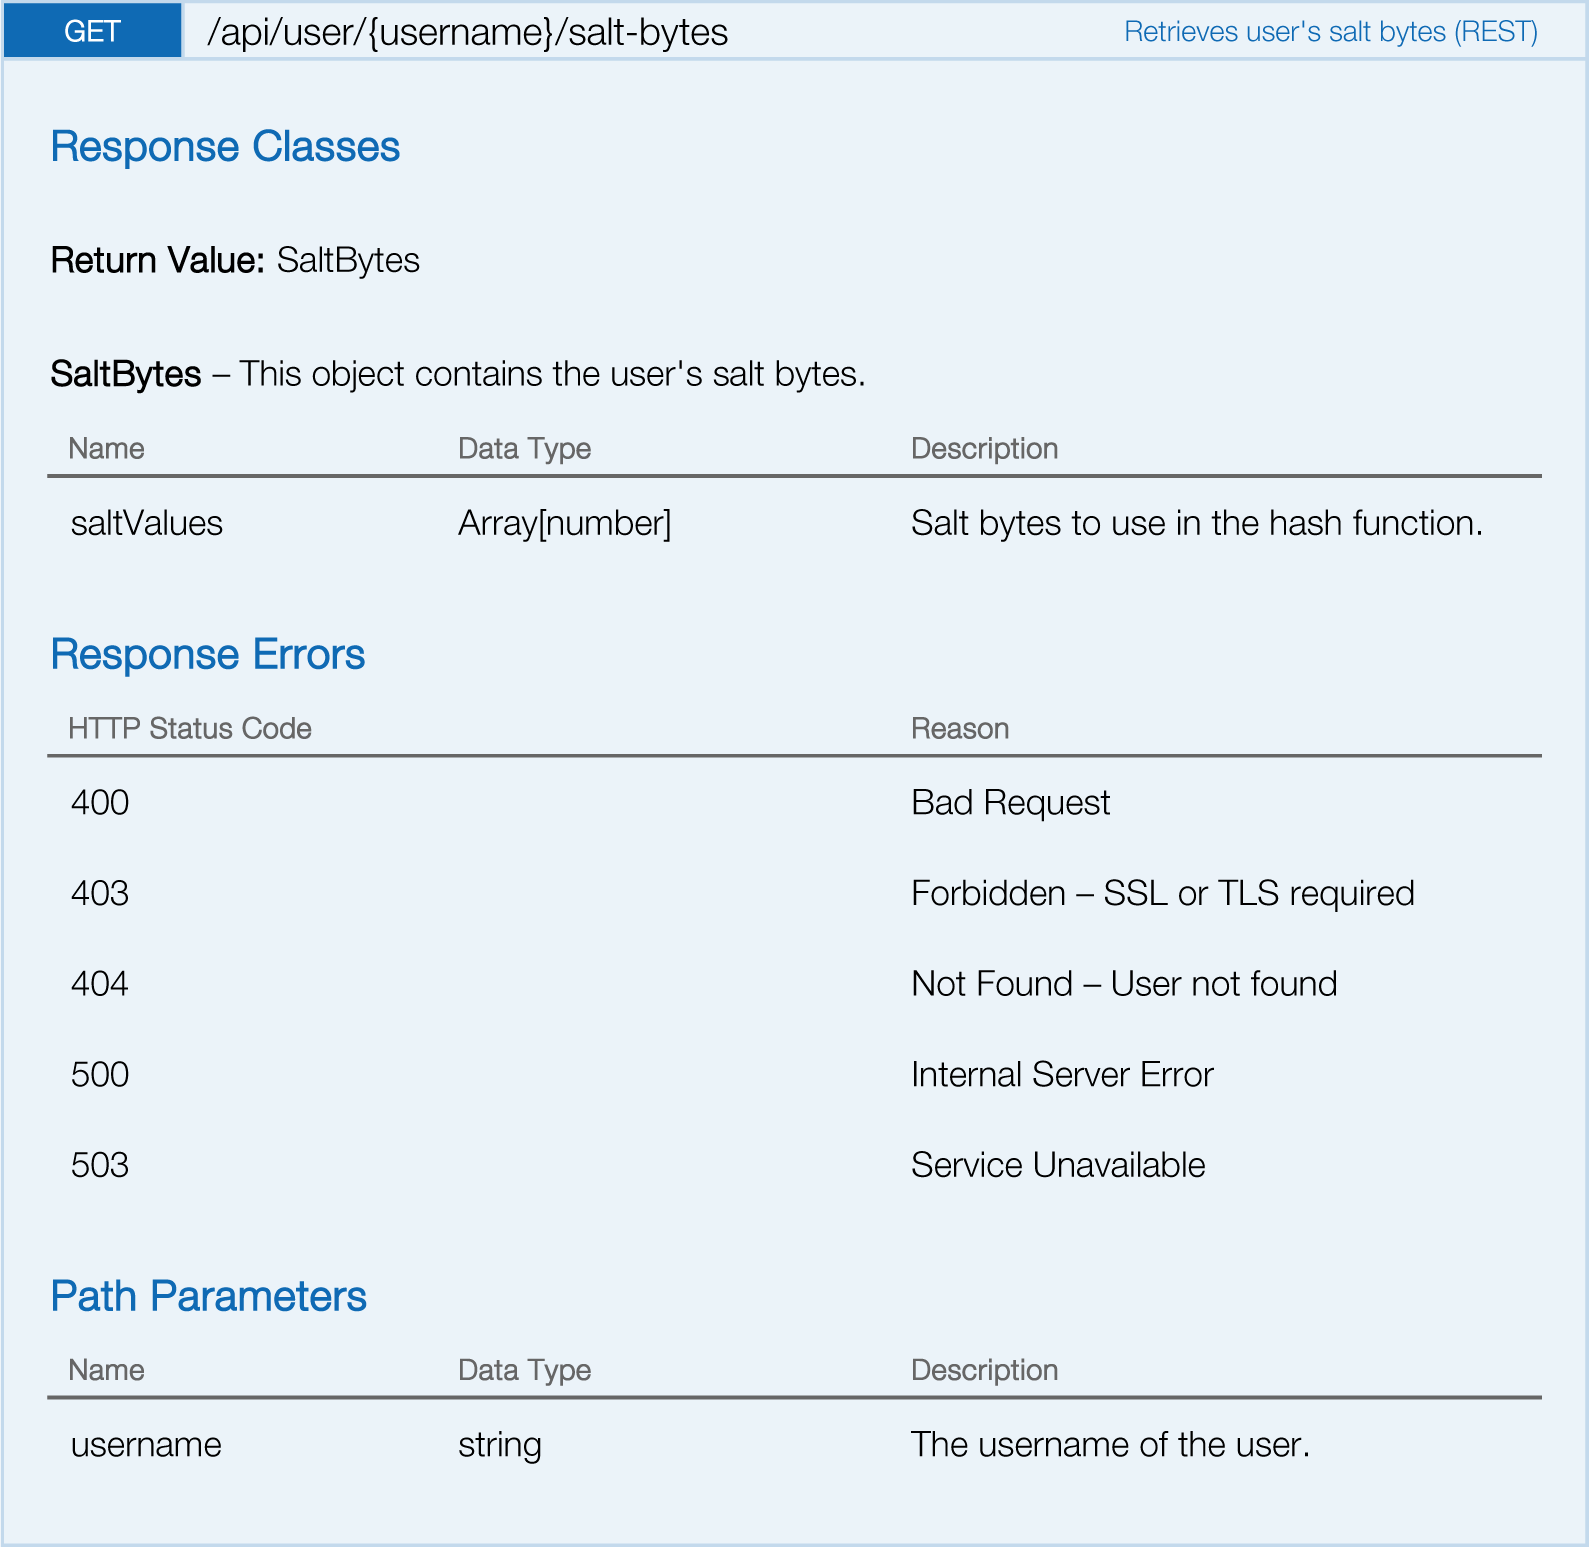
\includegraphics{apitables/APISaltBytes.png}
    	\label{fig:api-salt-bytes}
\end{figure}

\subsubsubsection{[User] Deletes user}
\begin{figure}[H]
	\noindent
    	\centering
    	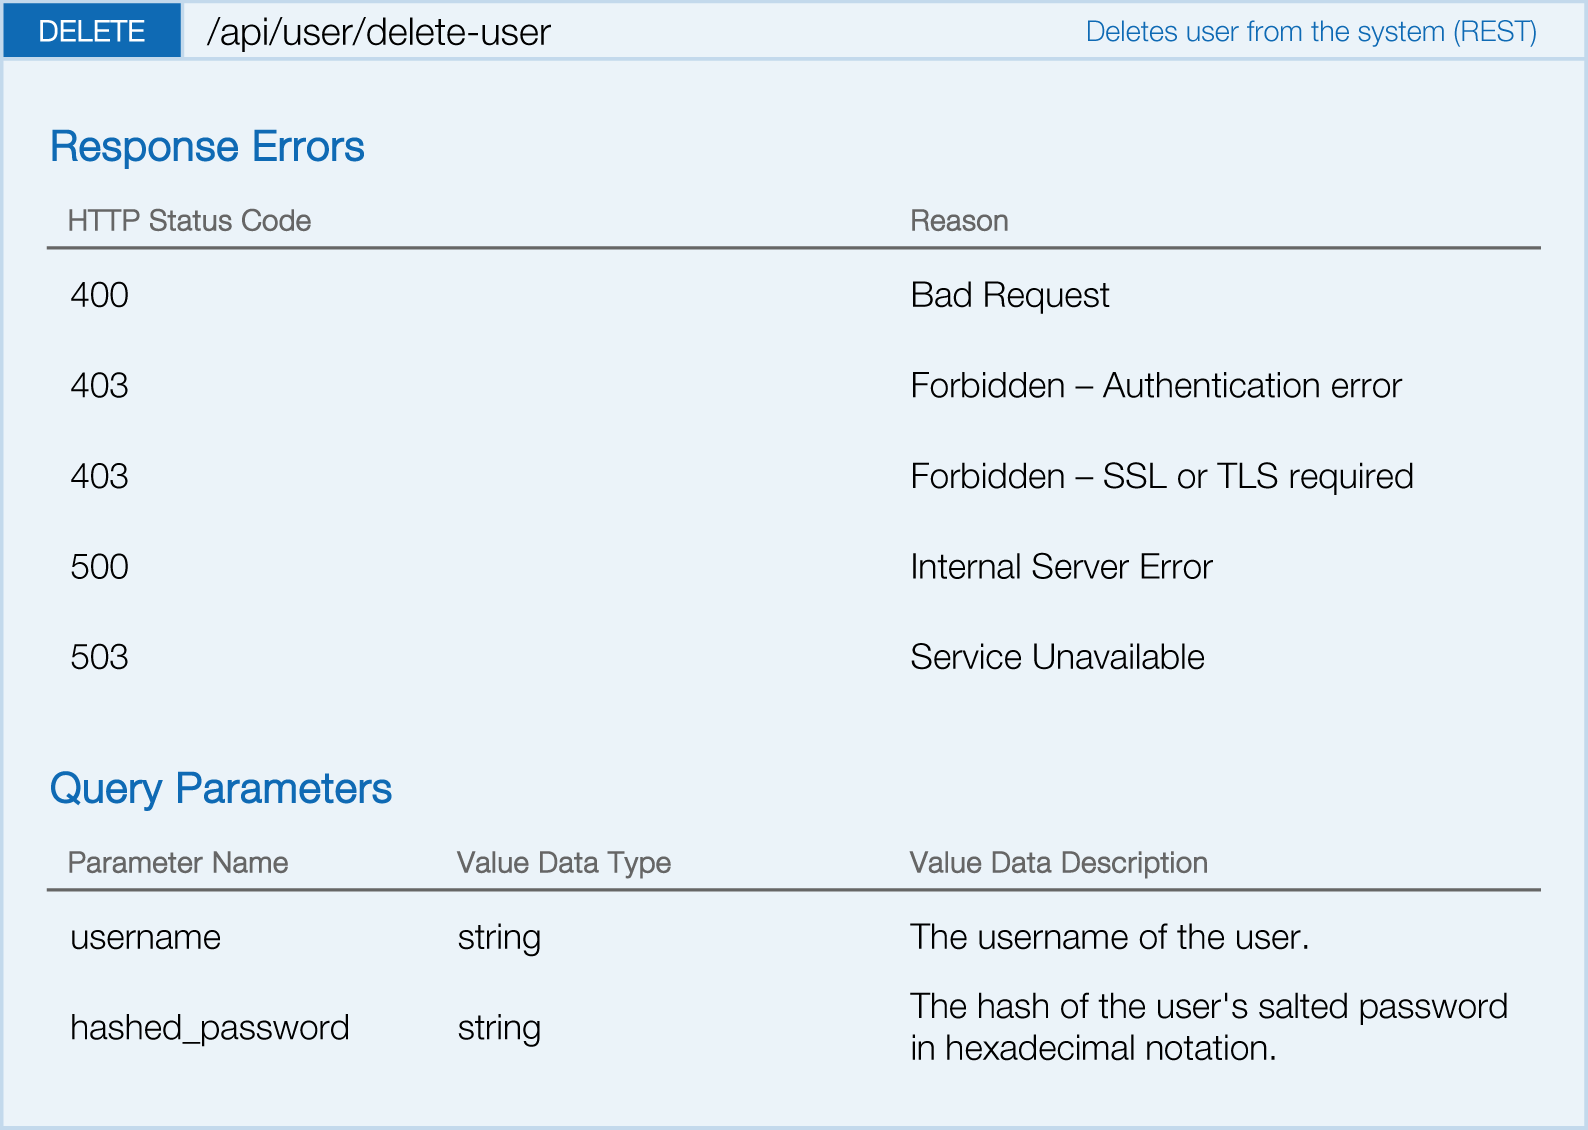
\includegraphics{apitables/APIDeleteUser.png}
    	\label{fig:api-delete-user}
\end{figure}

\subsubsubsection{[User] Retrieves user's rental logbook}
\begin{figure}[H]
	\noindent
    	\centering 
    	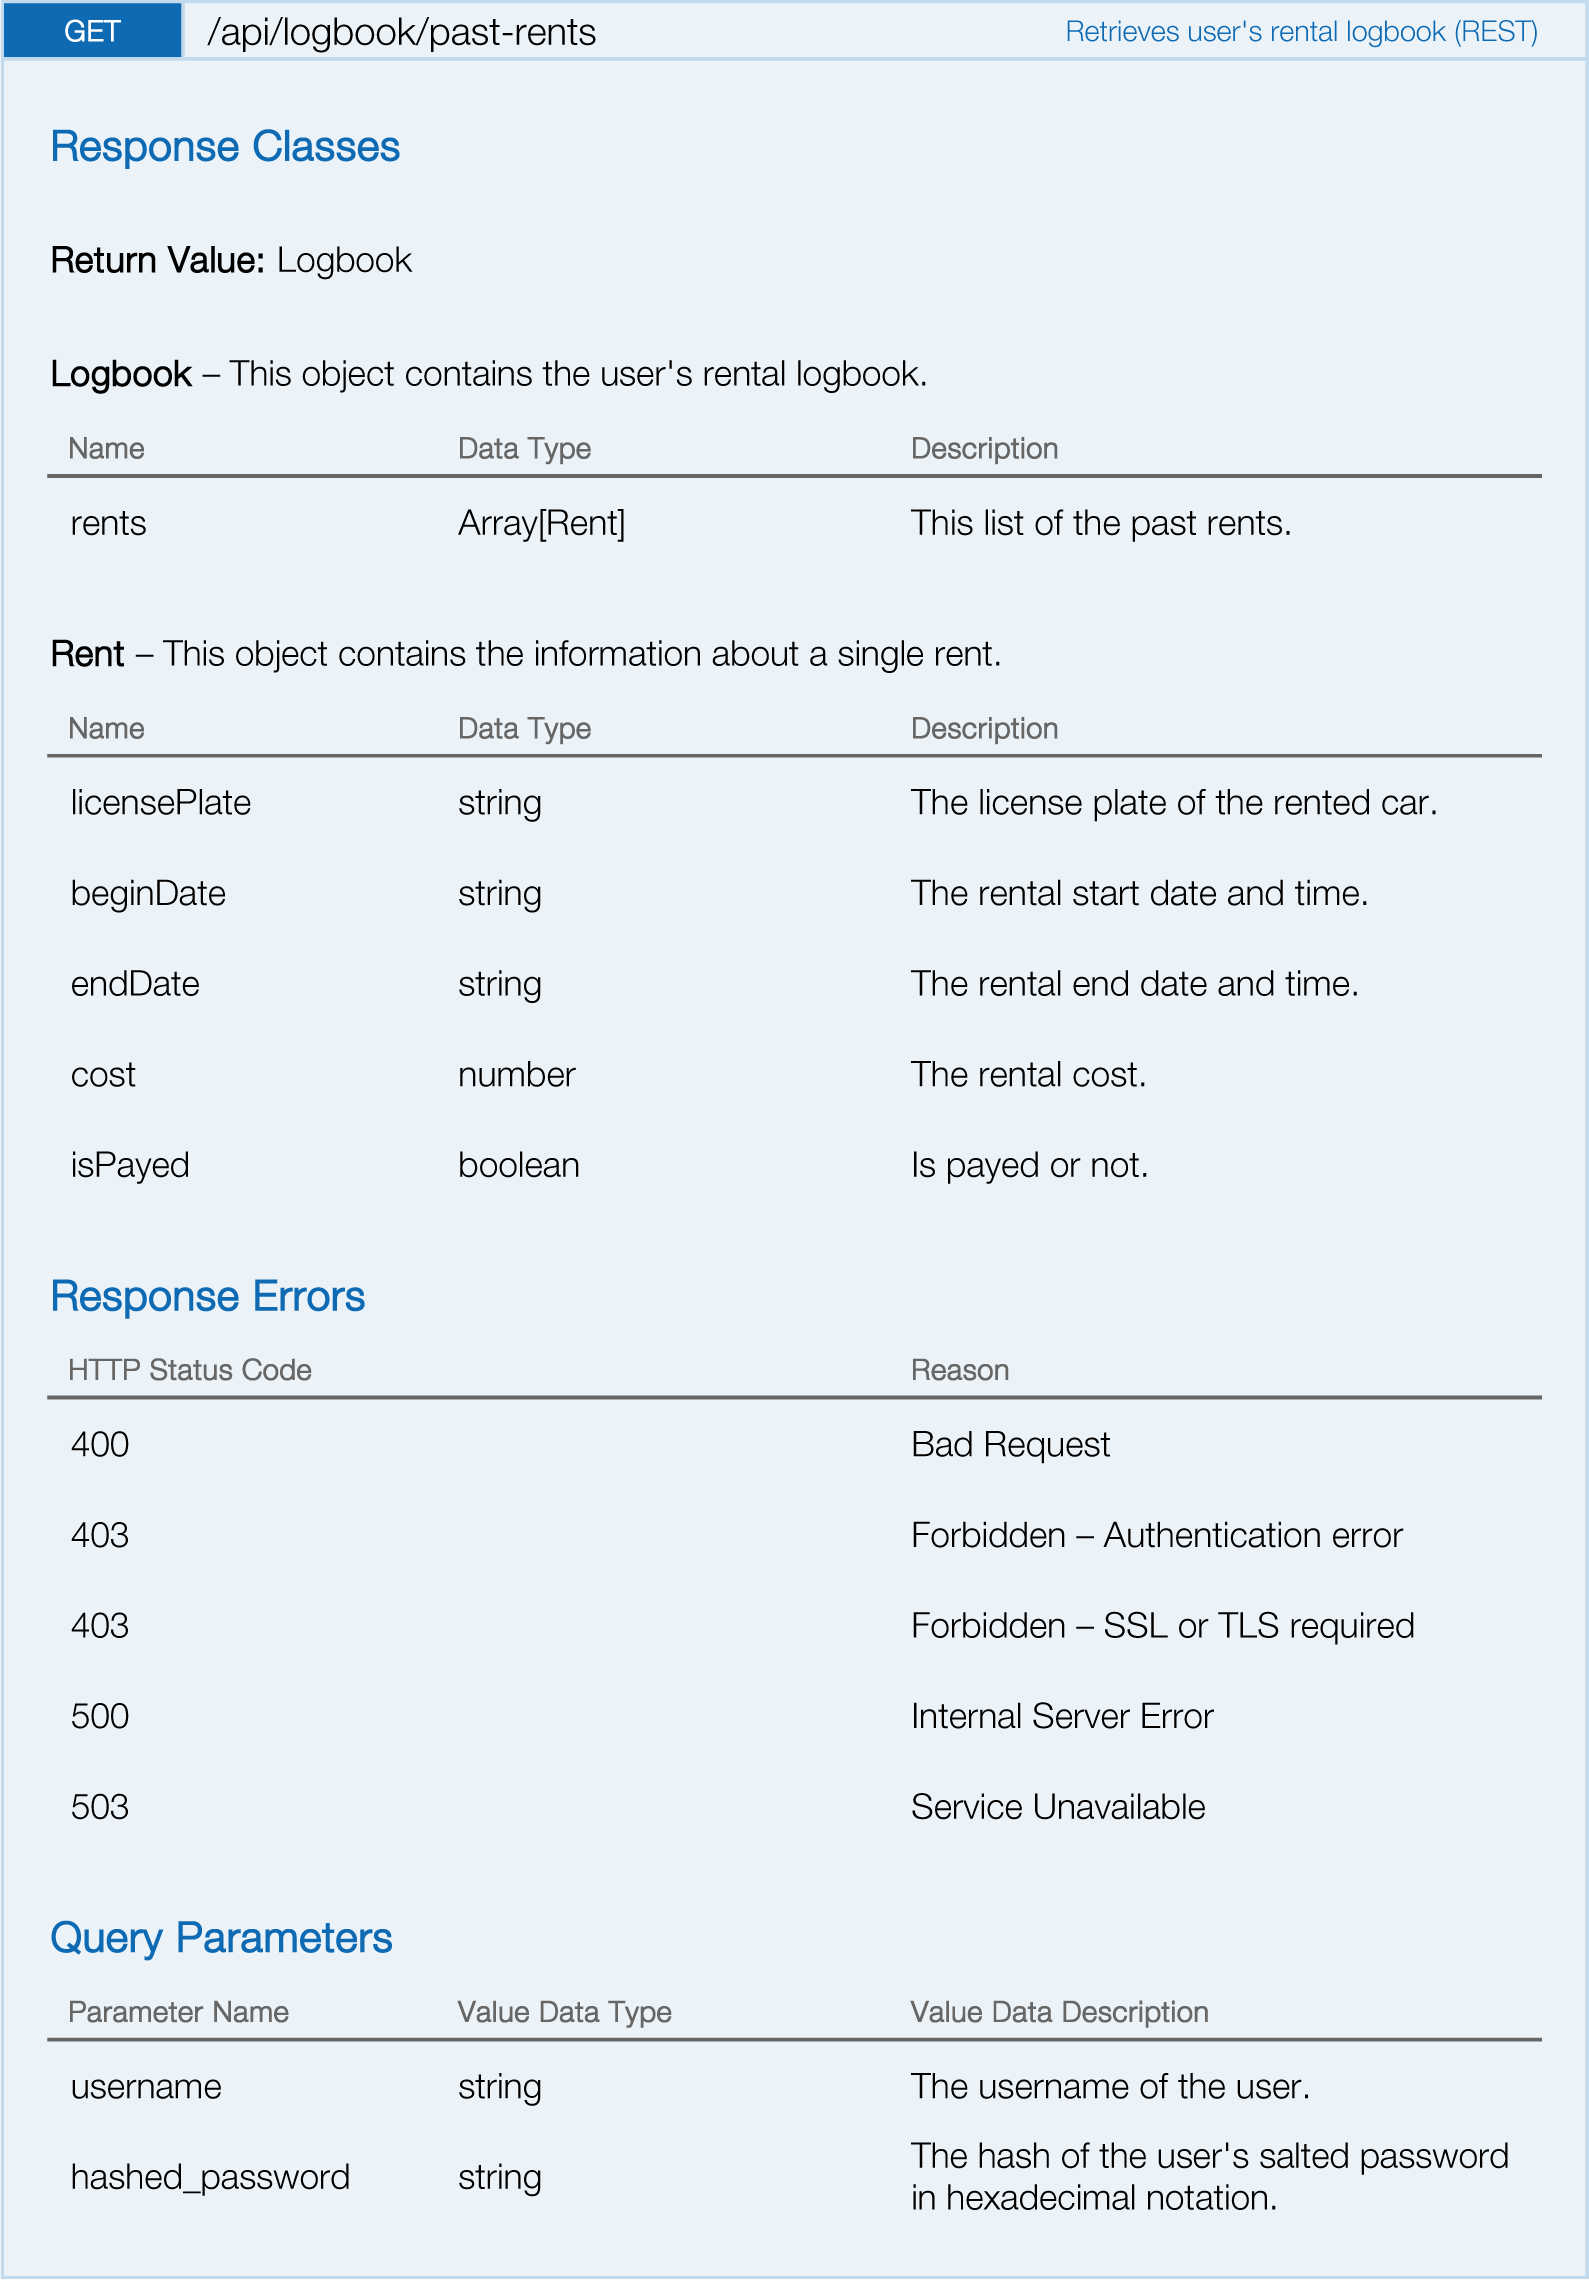
\includegraphics{apitables/APIPastRents.png}
    	\label{fig:api-past-rents}
\end{figure}

\subsubsubsection{[User]Retrieves available cars}
\begin{figure}[H]
	\noindent
    	\centering
    	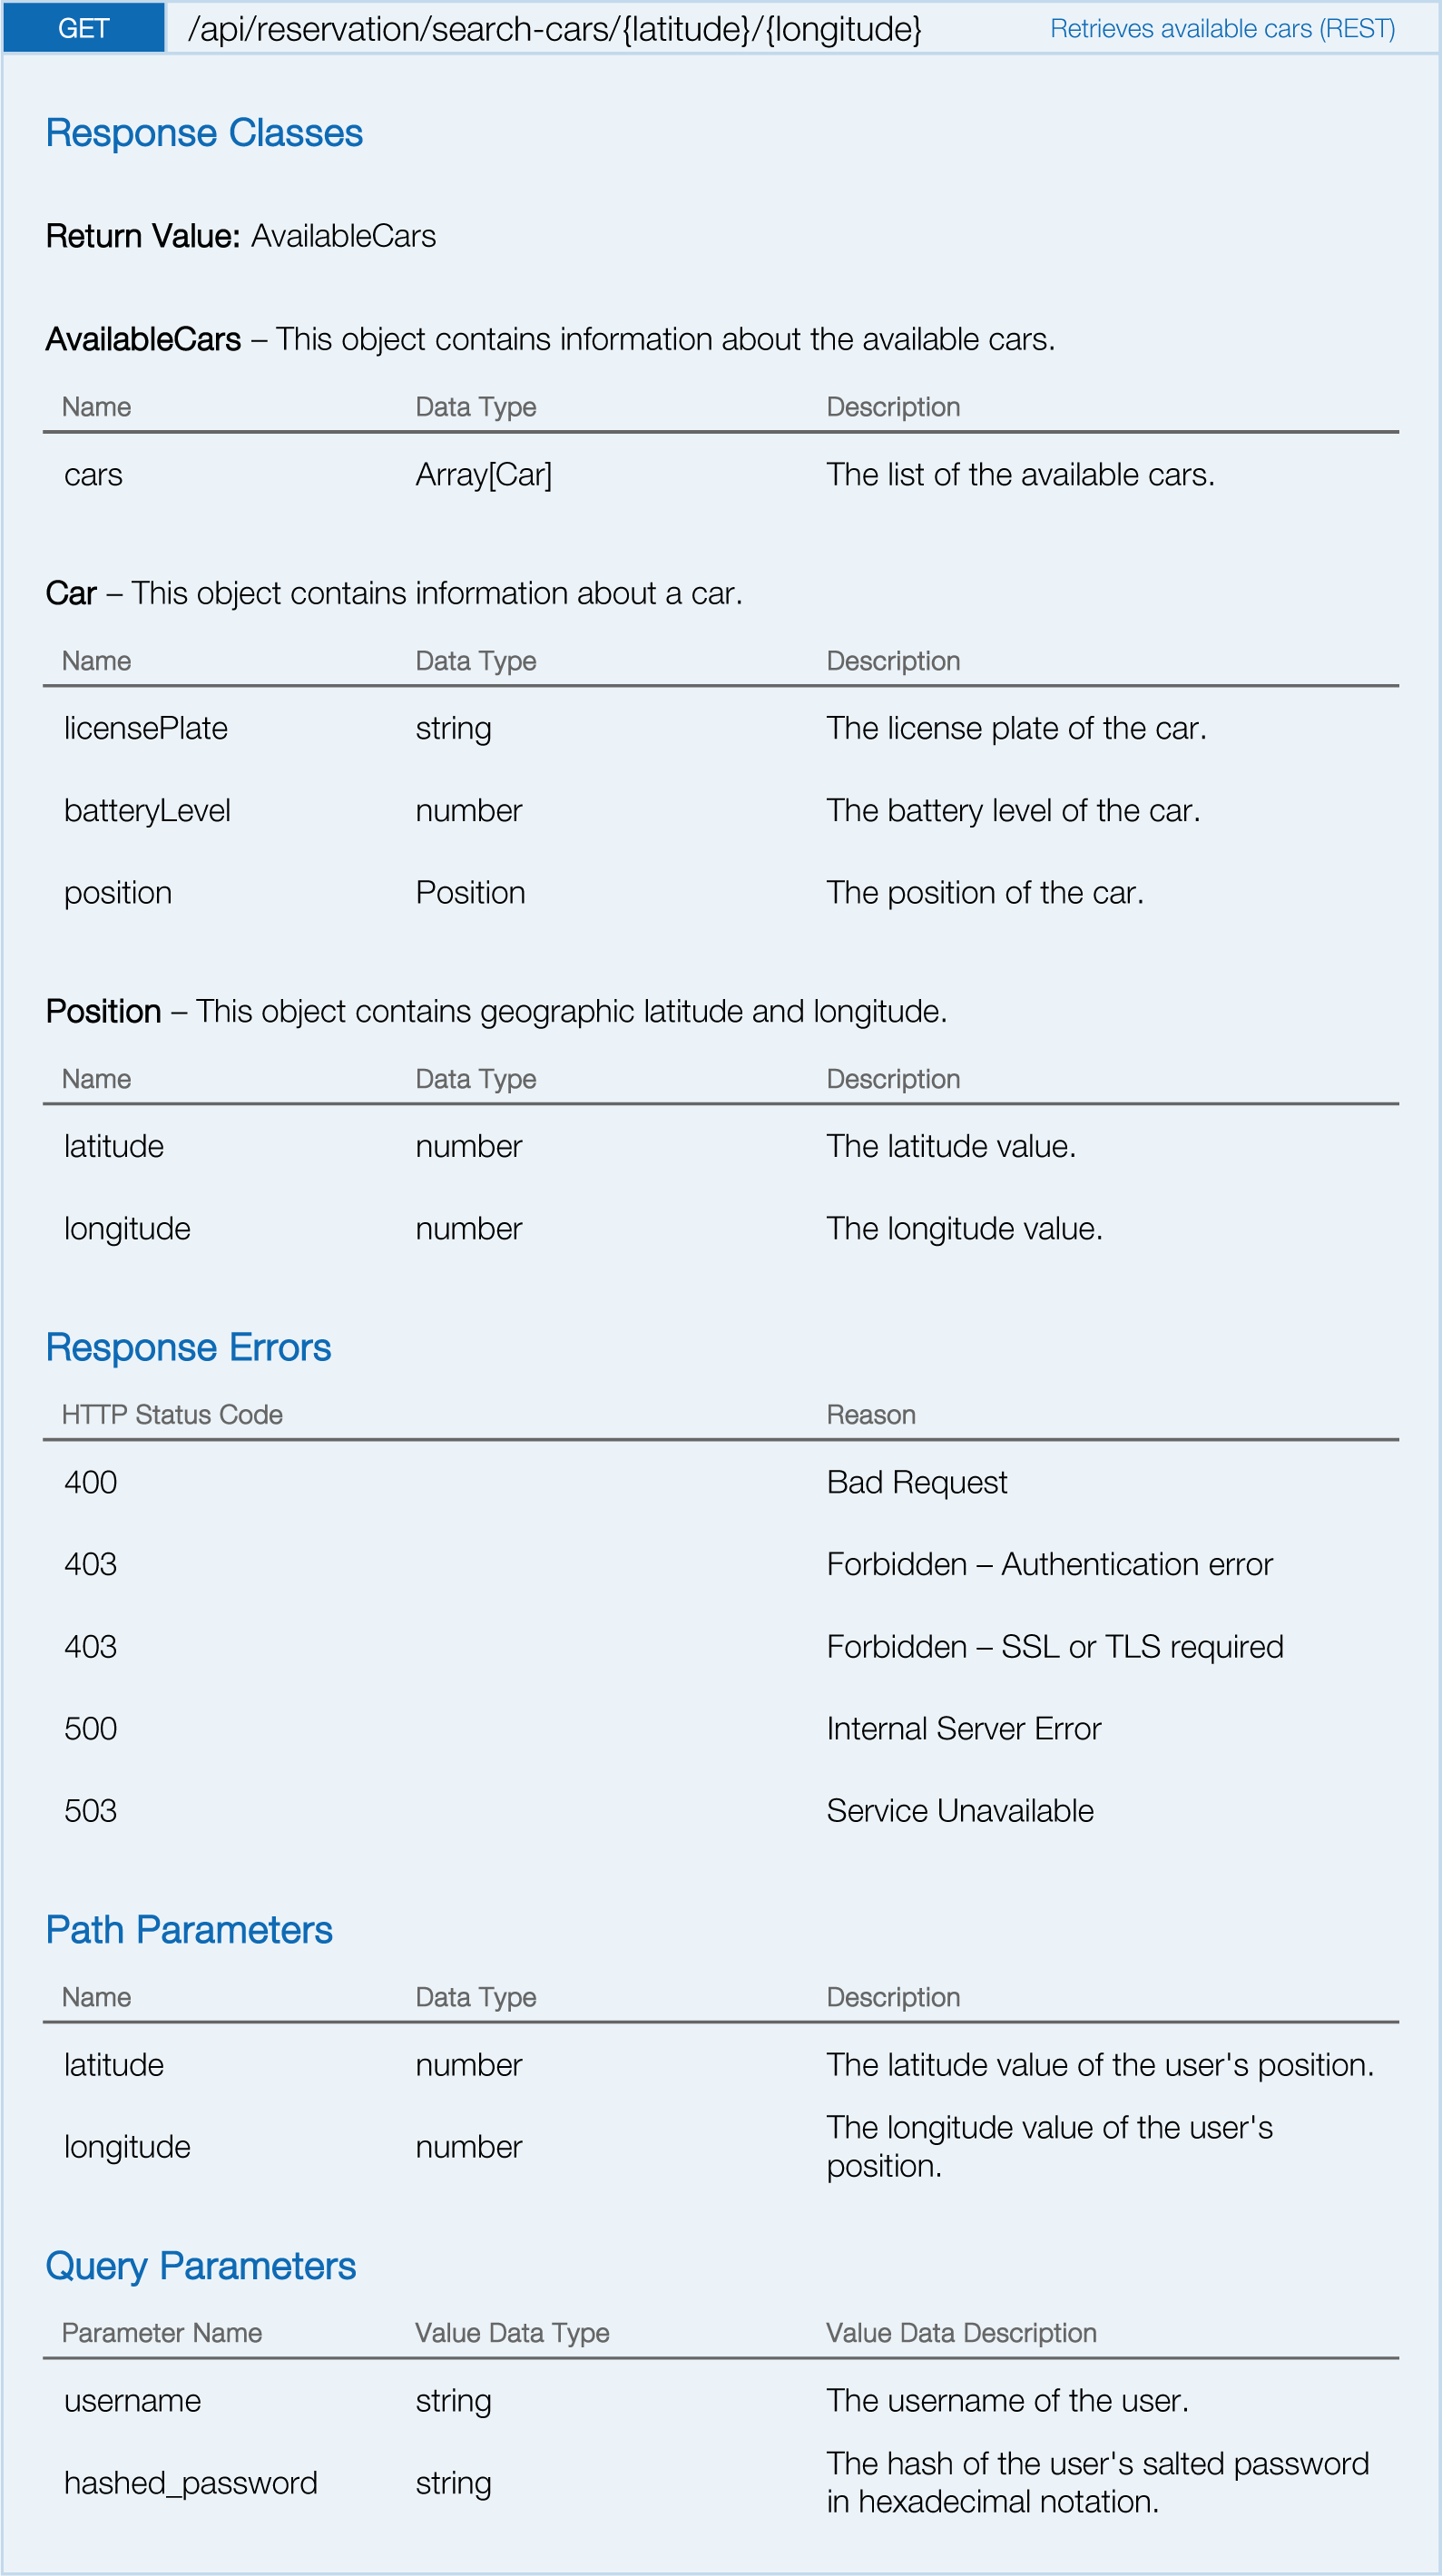
\includegraphics[height=550px, keepaspectratio]{apitables/APISearchCars.png}
    	\label{fig:api-search-cars}
\end{figure}

\subsubsubsection{[User] Reserves car}
\begin{figure}[H]
	\noindent
    	\centering
    	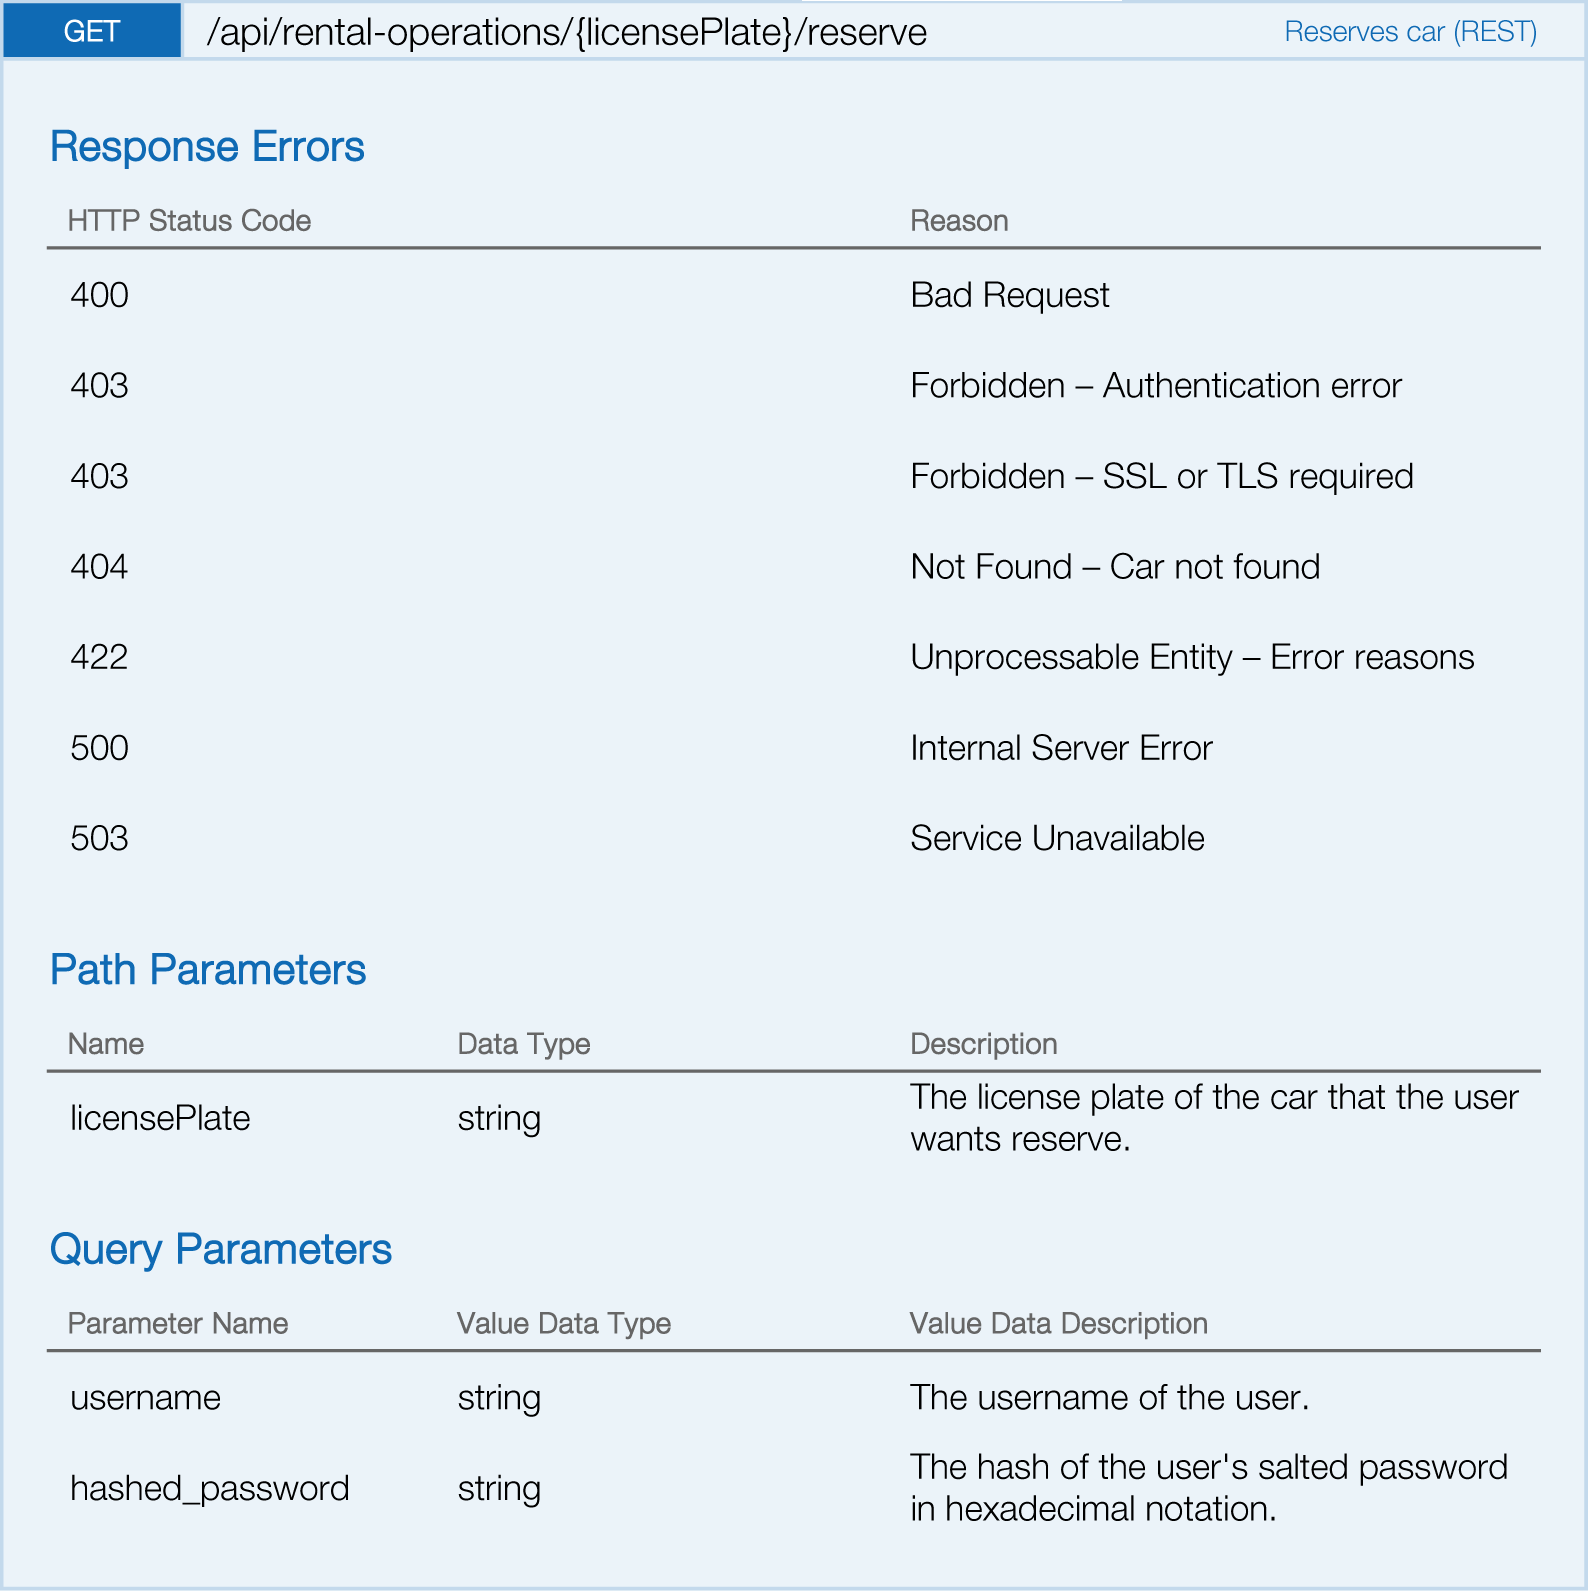
\includegraphics{apitables/APIReservation.png}
    	\label{fig:api-reservation}
\end{figure}

\subsubsubsection{[User] Retrieves current reservation}
\begin{figure}[H]
	\noindent
    	\centering
    	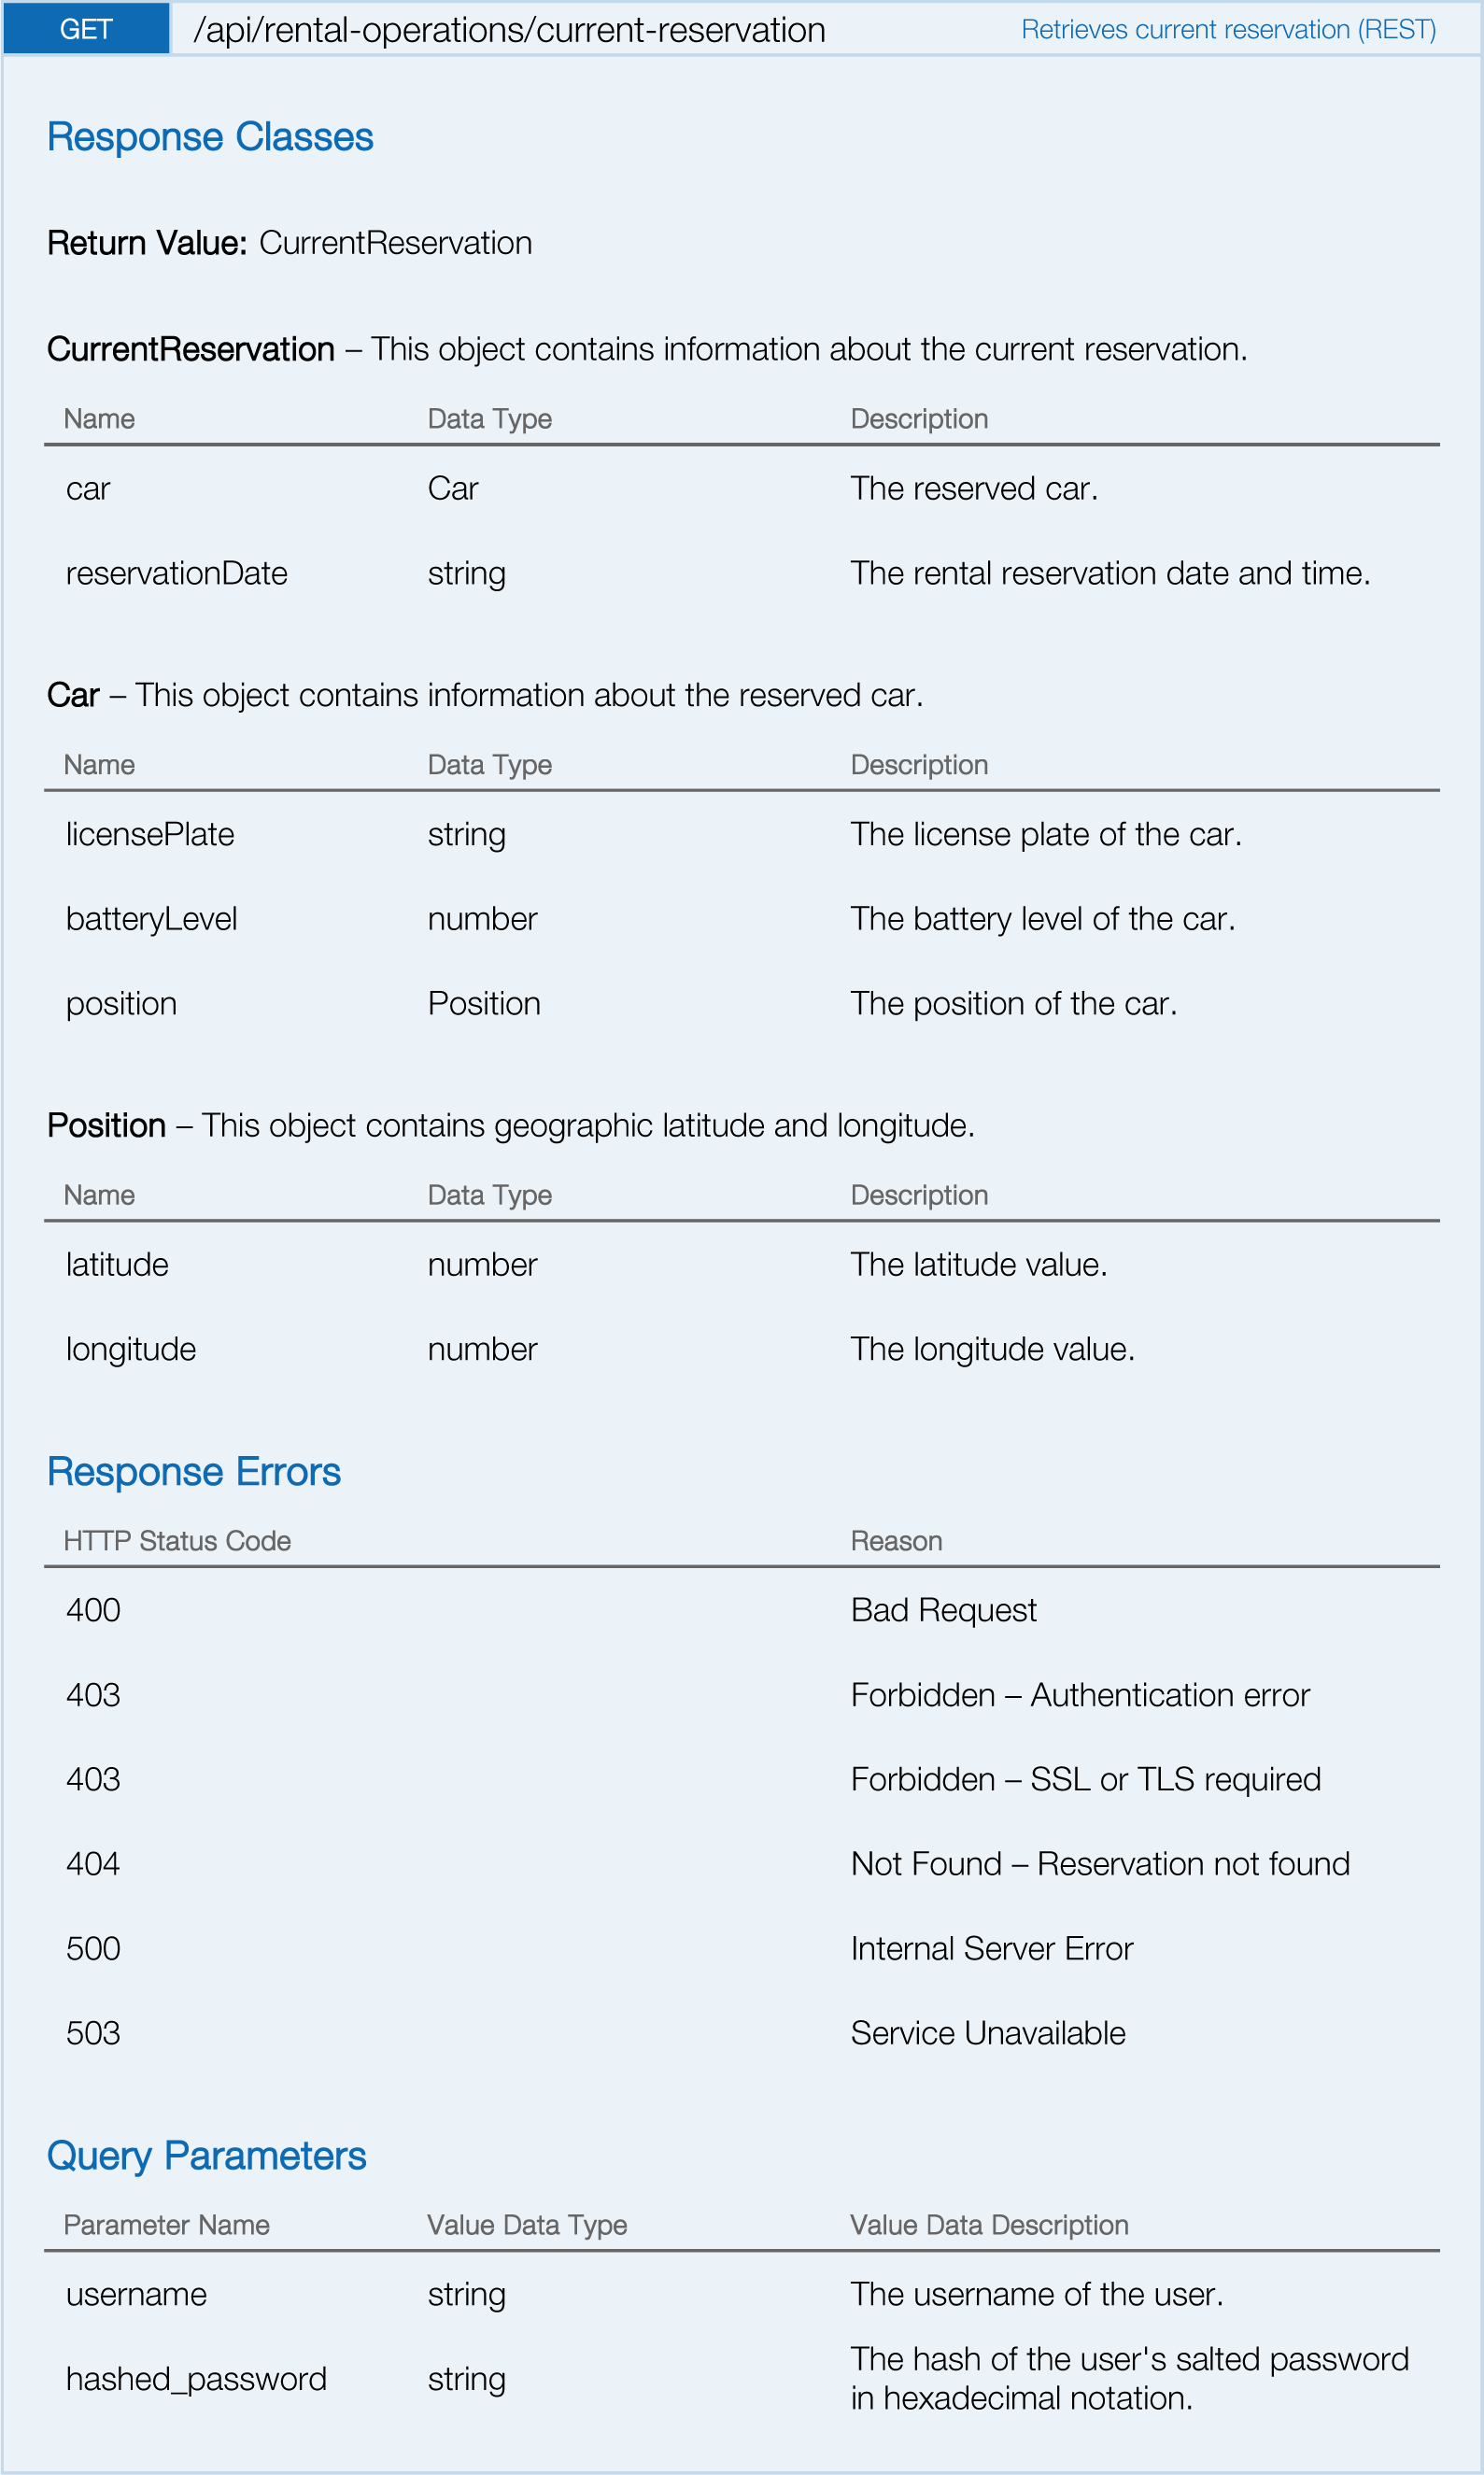
\includegraphics[height=550px, keepaspectratio]{apitables/APICurrentReservation.png}
    	\label{fig:api-current-reservation}
\end{figure}

\subsubsubsection{[User] Unlocks car}
\begin{figure}[H]
	\noindent
    	\centering
    	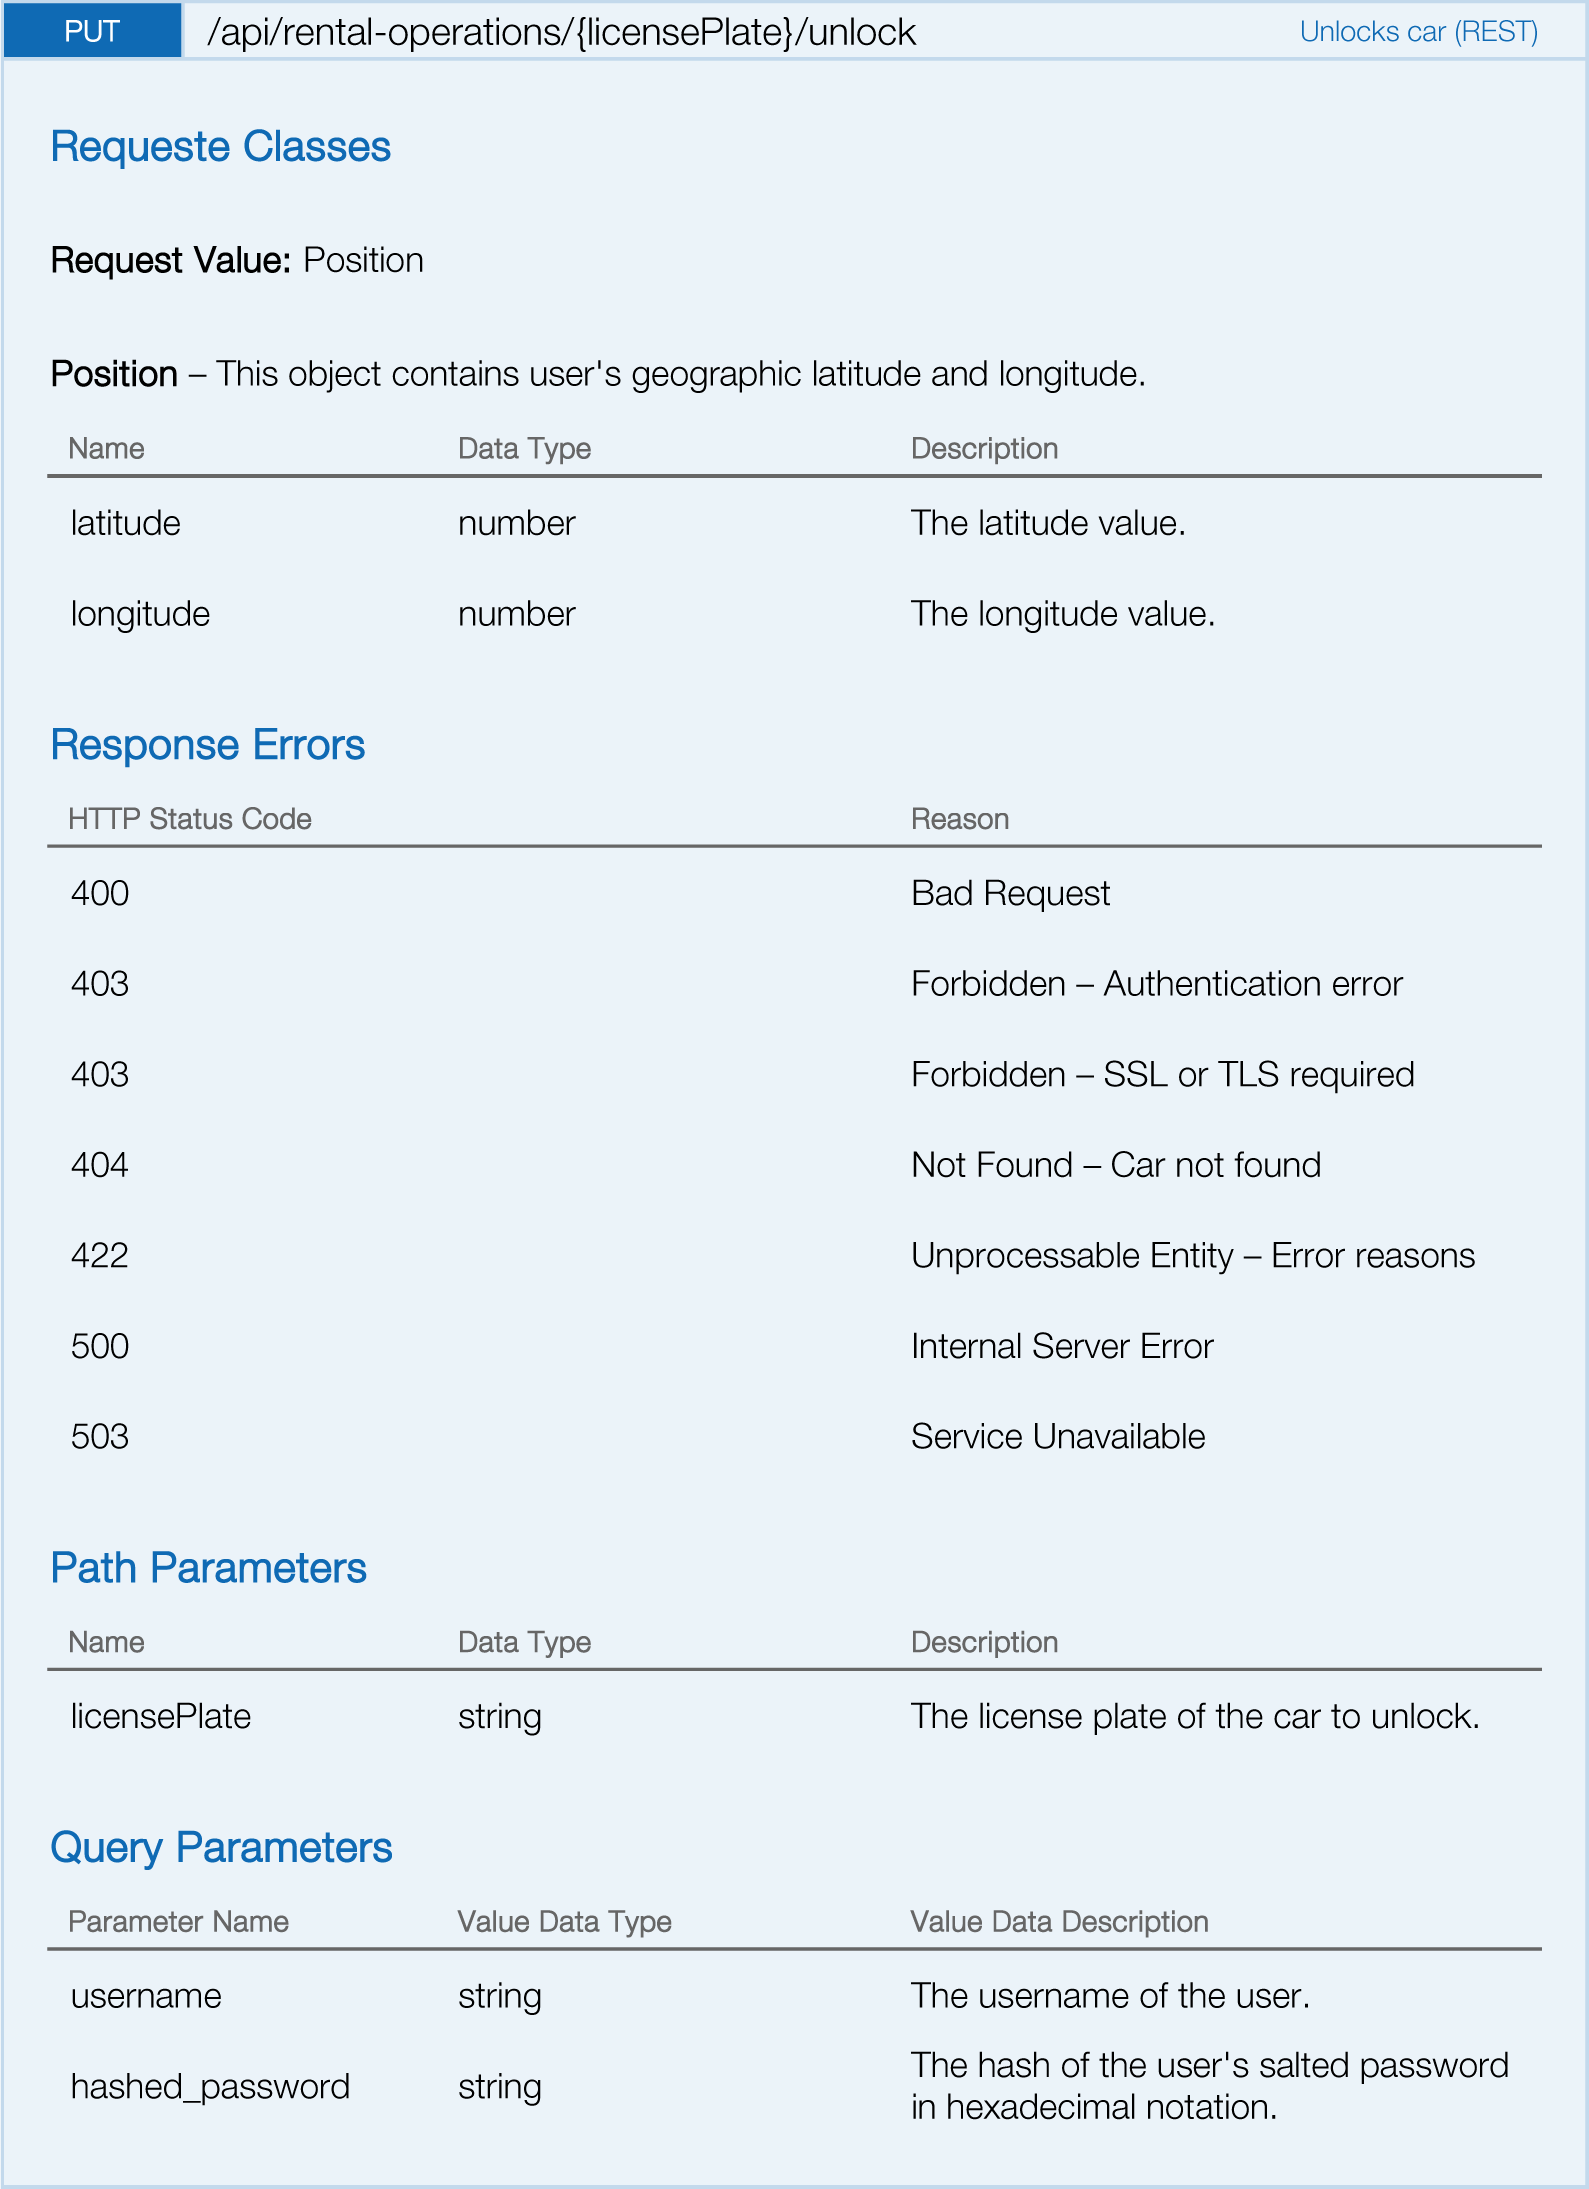
\includegraphics{apitables/APIUnlockCar.png}
    	\label{fig:api-unlock-car}
\end{figure}

\subsubsubsection{[Car] Car Heartbeat}
\begin{figure}[H]
	\noindent
    	\centering
    	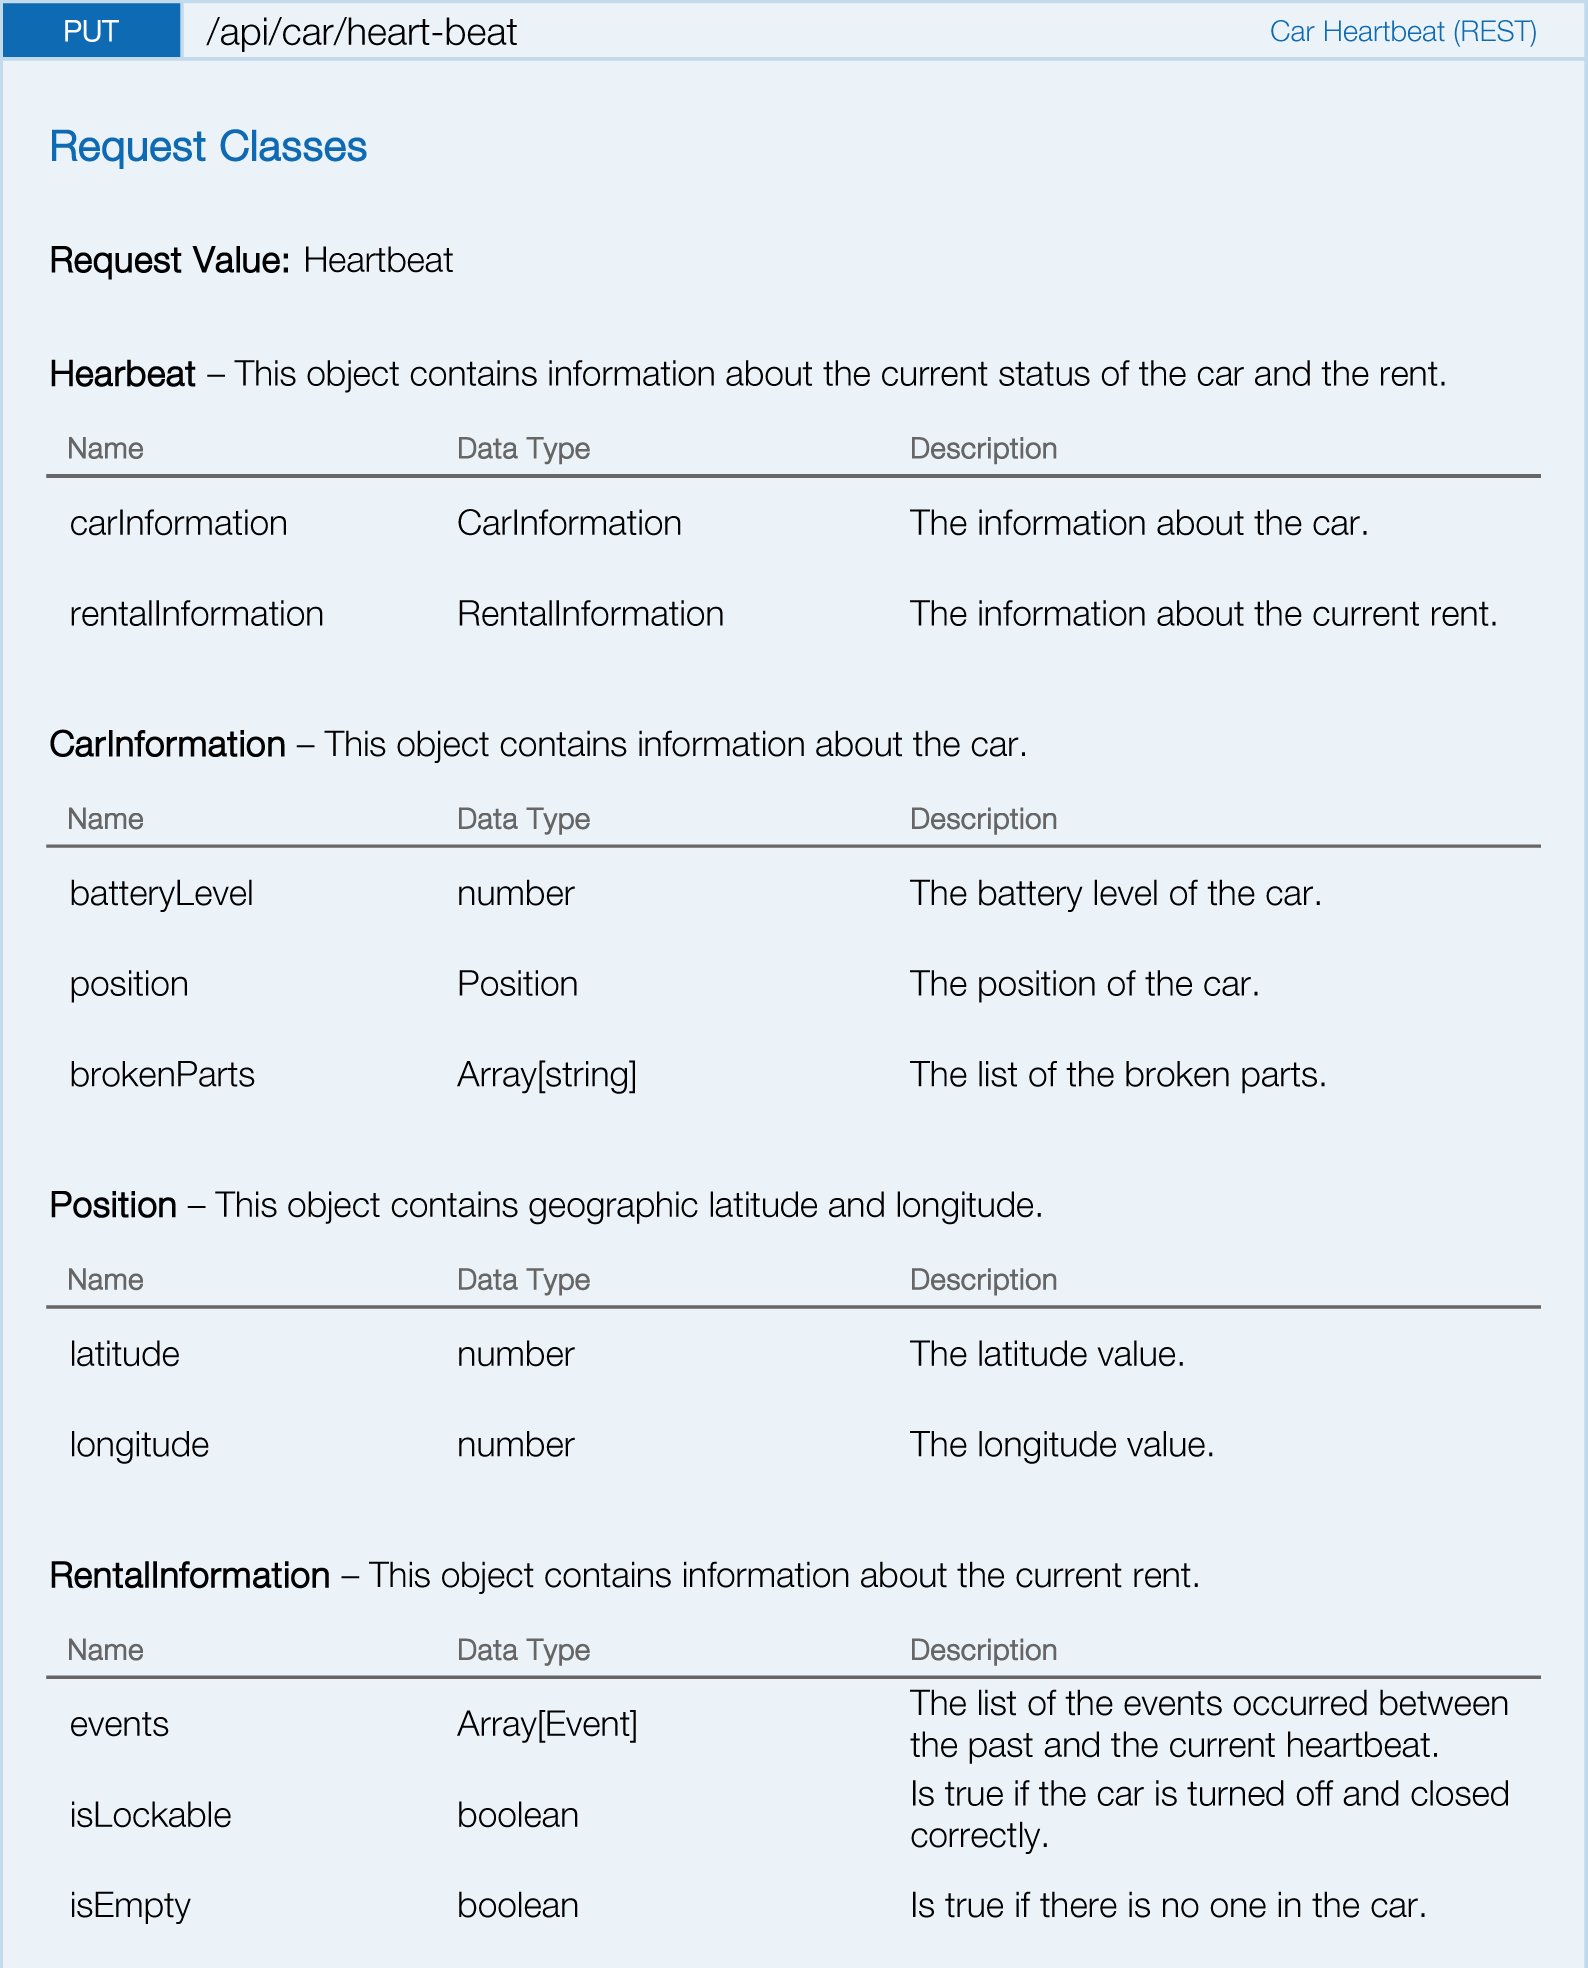
\includegraphics{apitables/APIHeartbeat1.png}
    	\label{fig:api-car-heartbeat1}
\end{figure}

\begin{figure}[H]
	\noindent
    	\centering
    	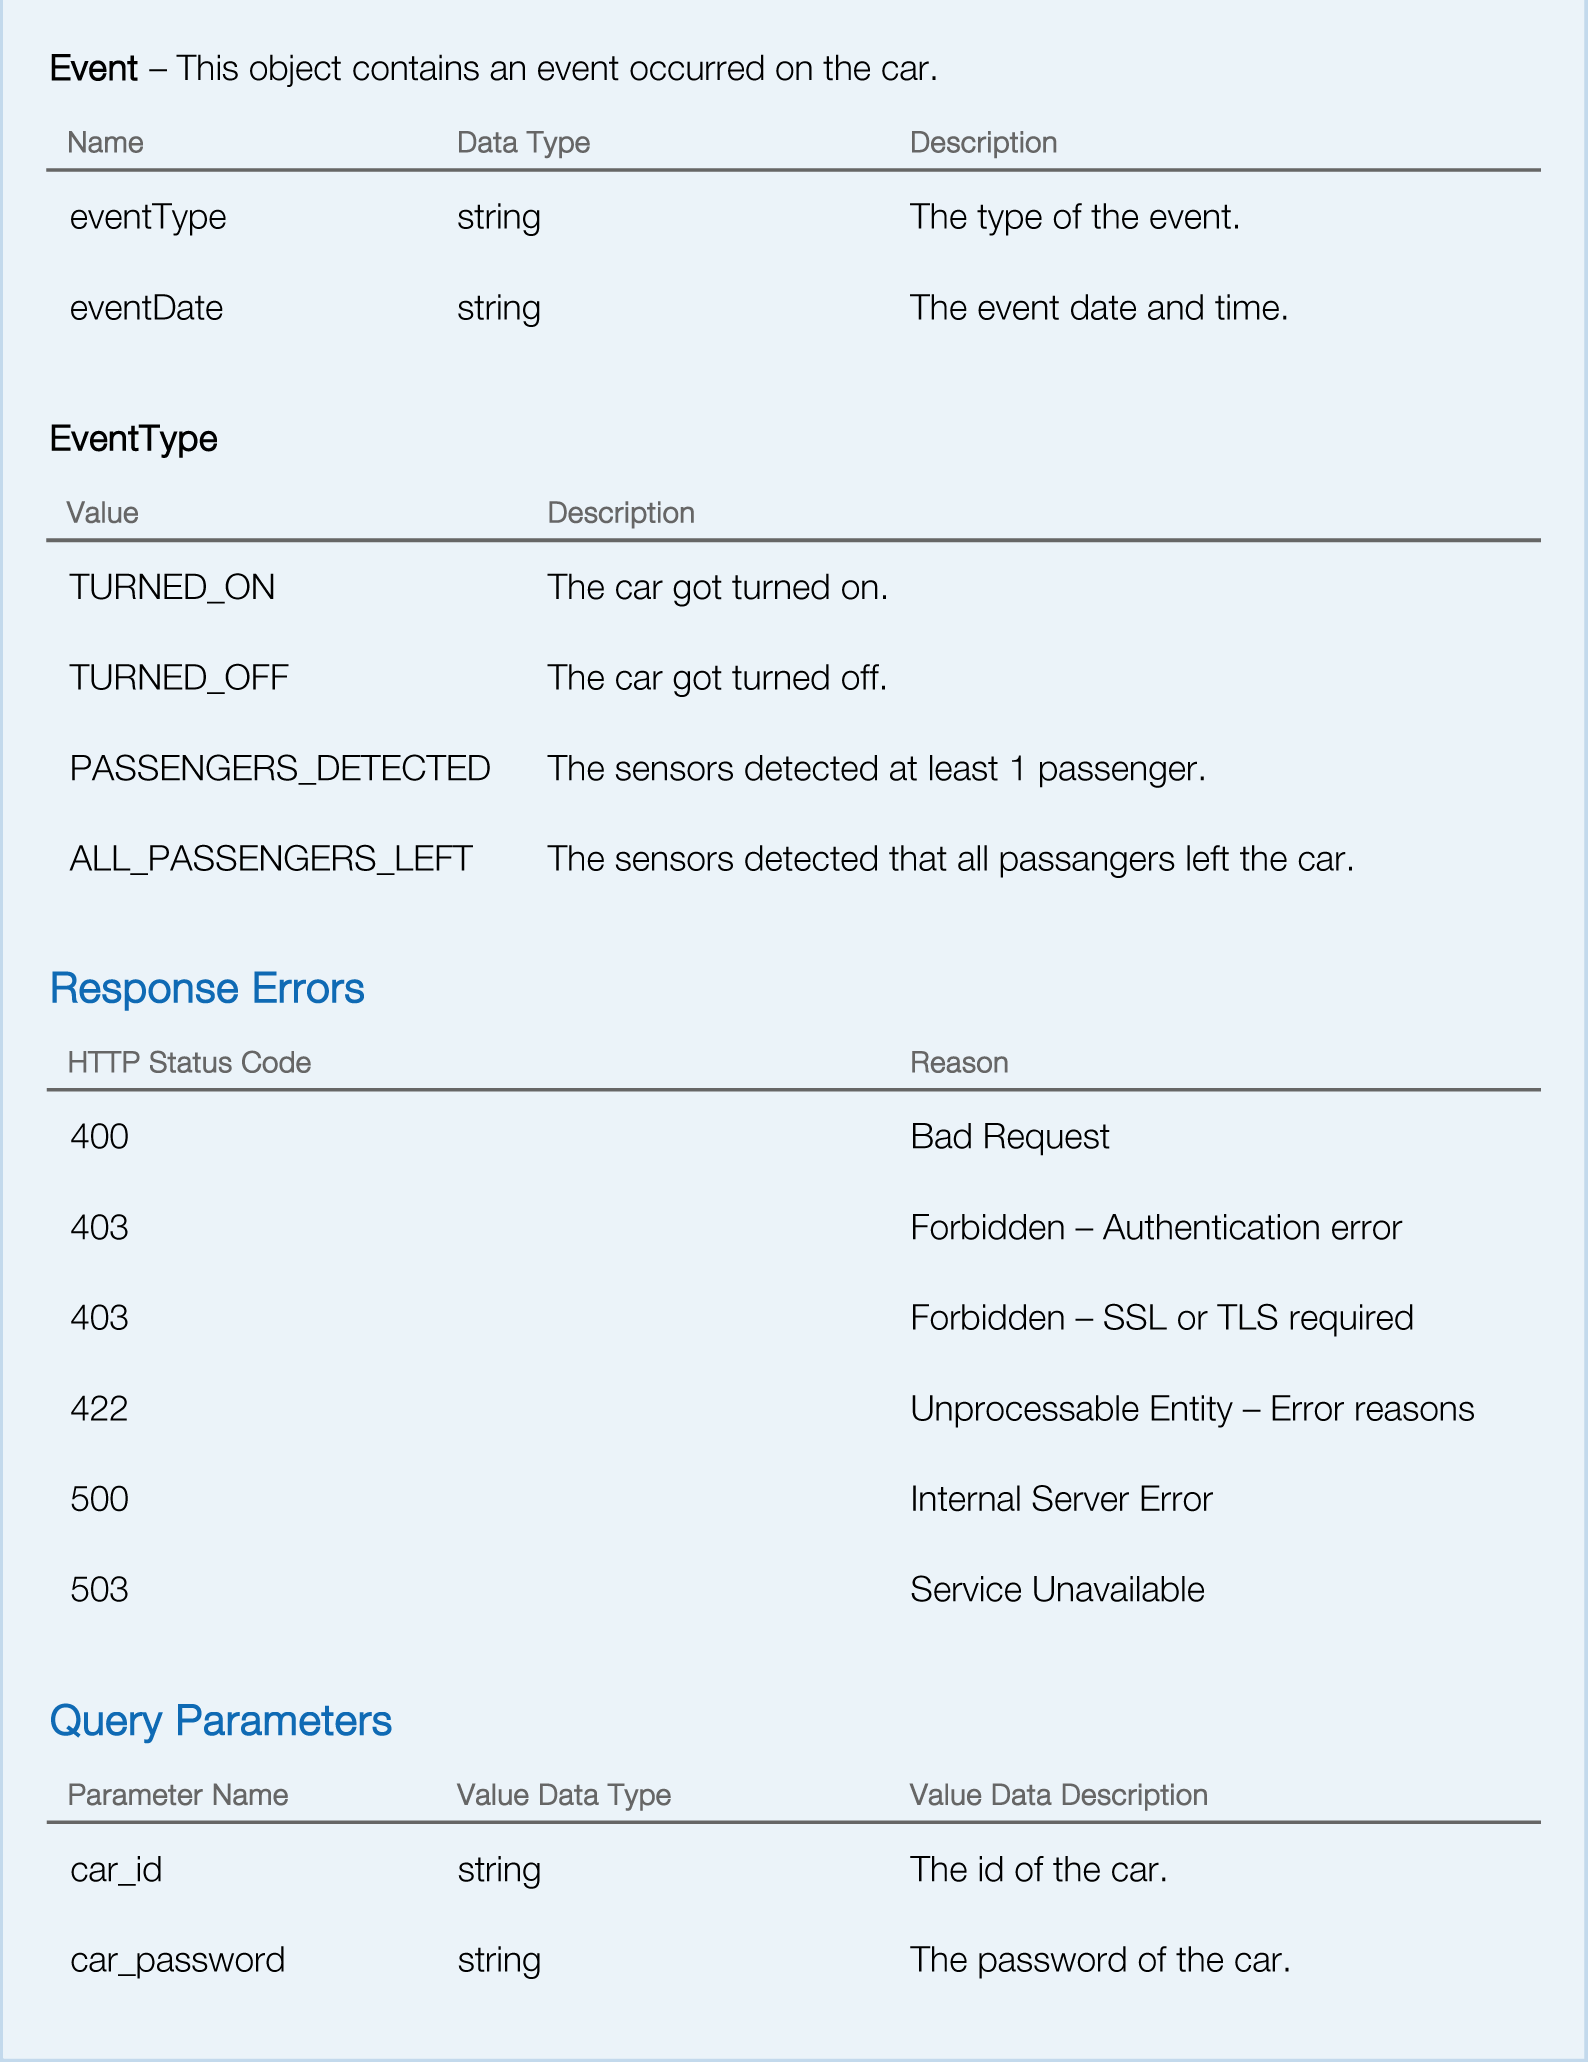
\includegraphics{apitables/APIHeartbeat2.png}
    	\label{fig:api-car-heartbeat2}
\end{figure}

\subsubsubsection{[Car] Retrieves available safe areas}
\begin{figure}[H]
	\noindent
    	\centering
    	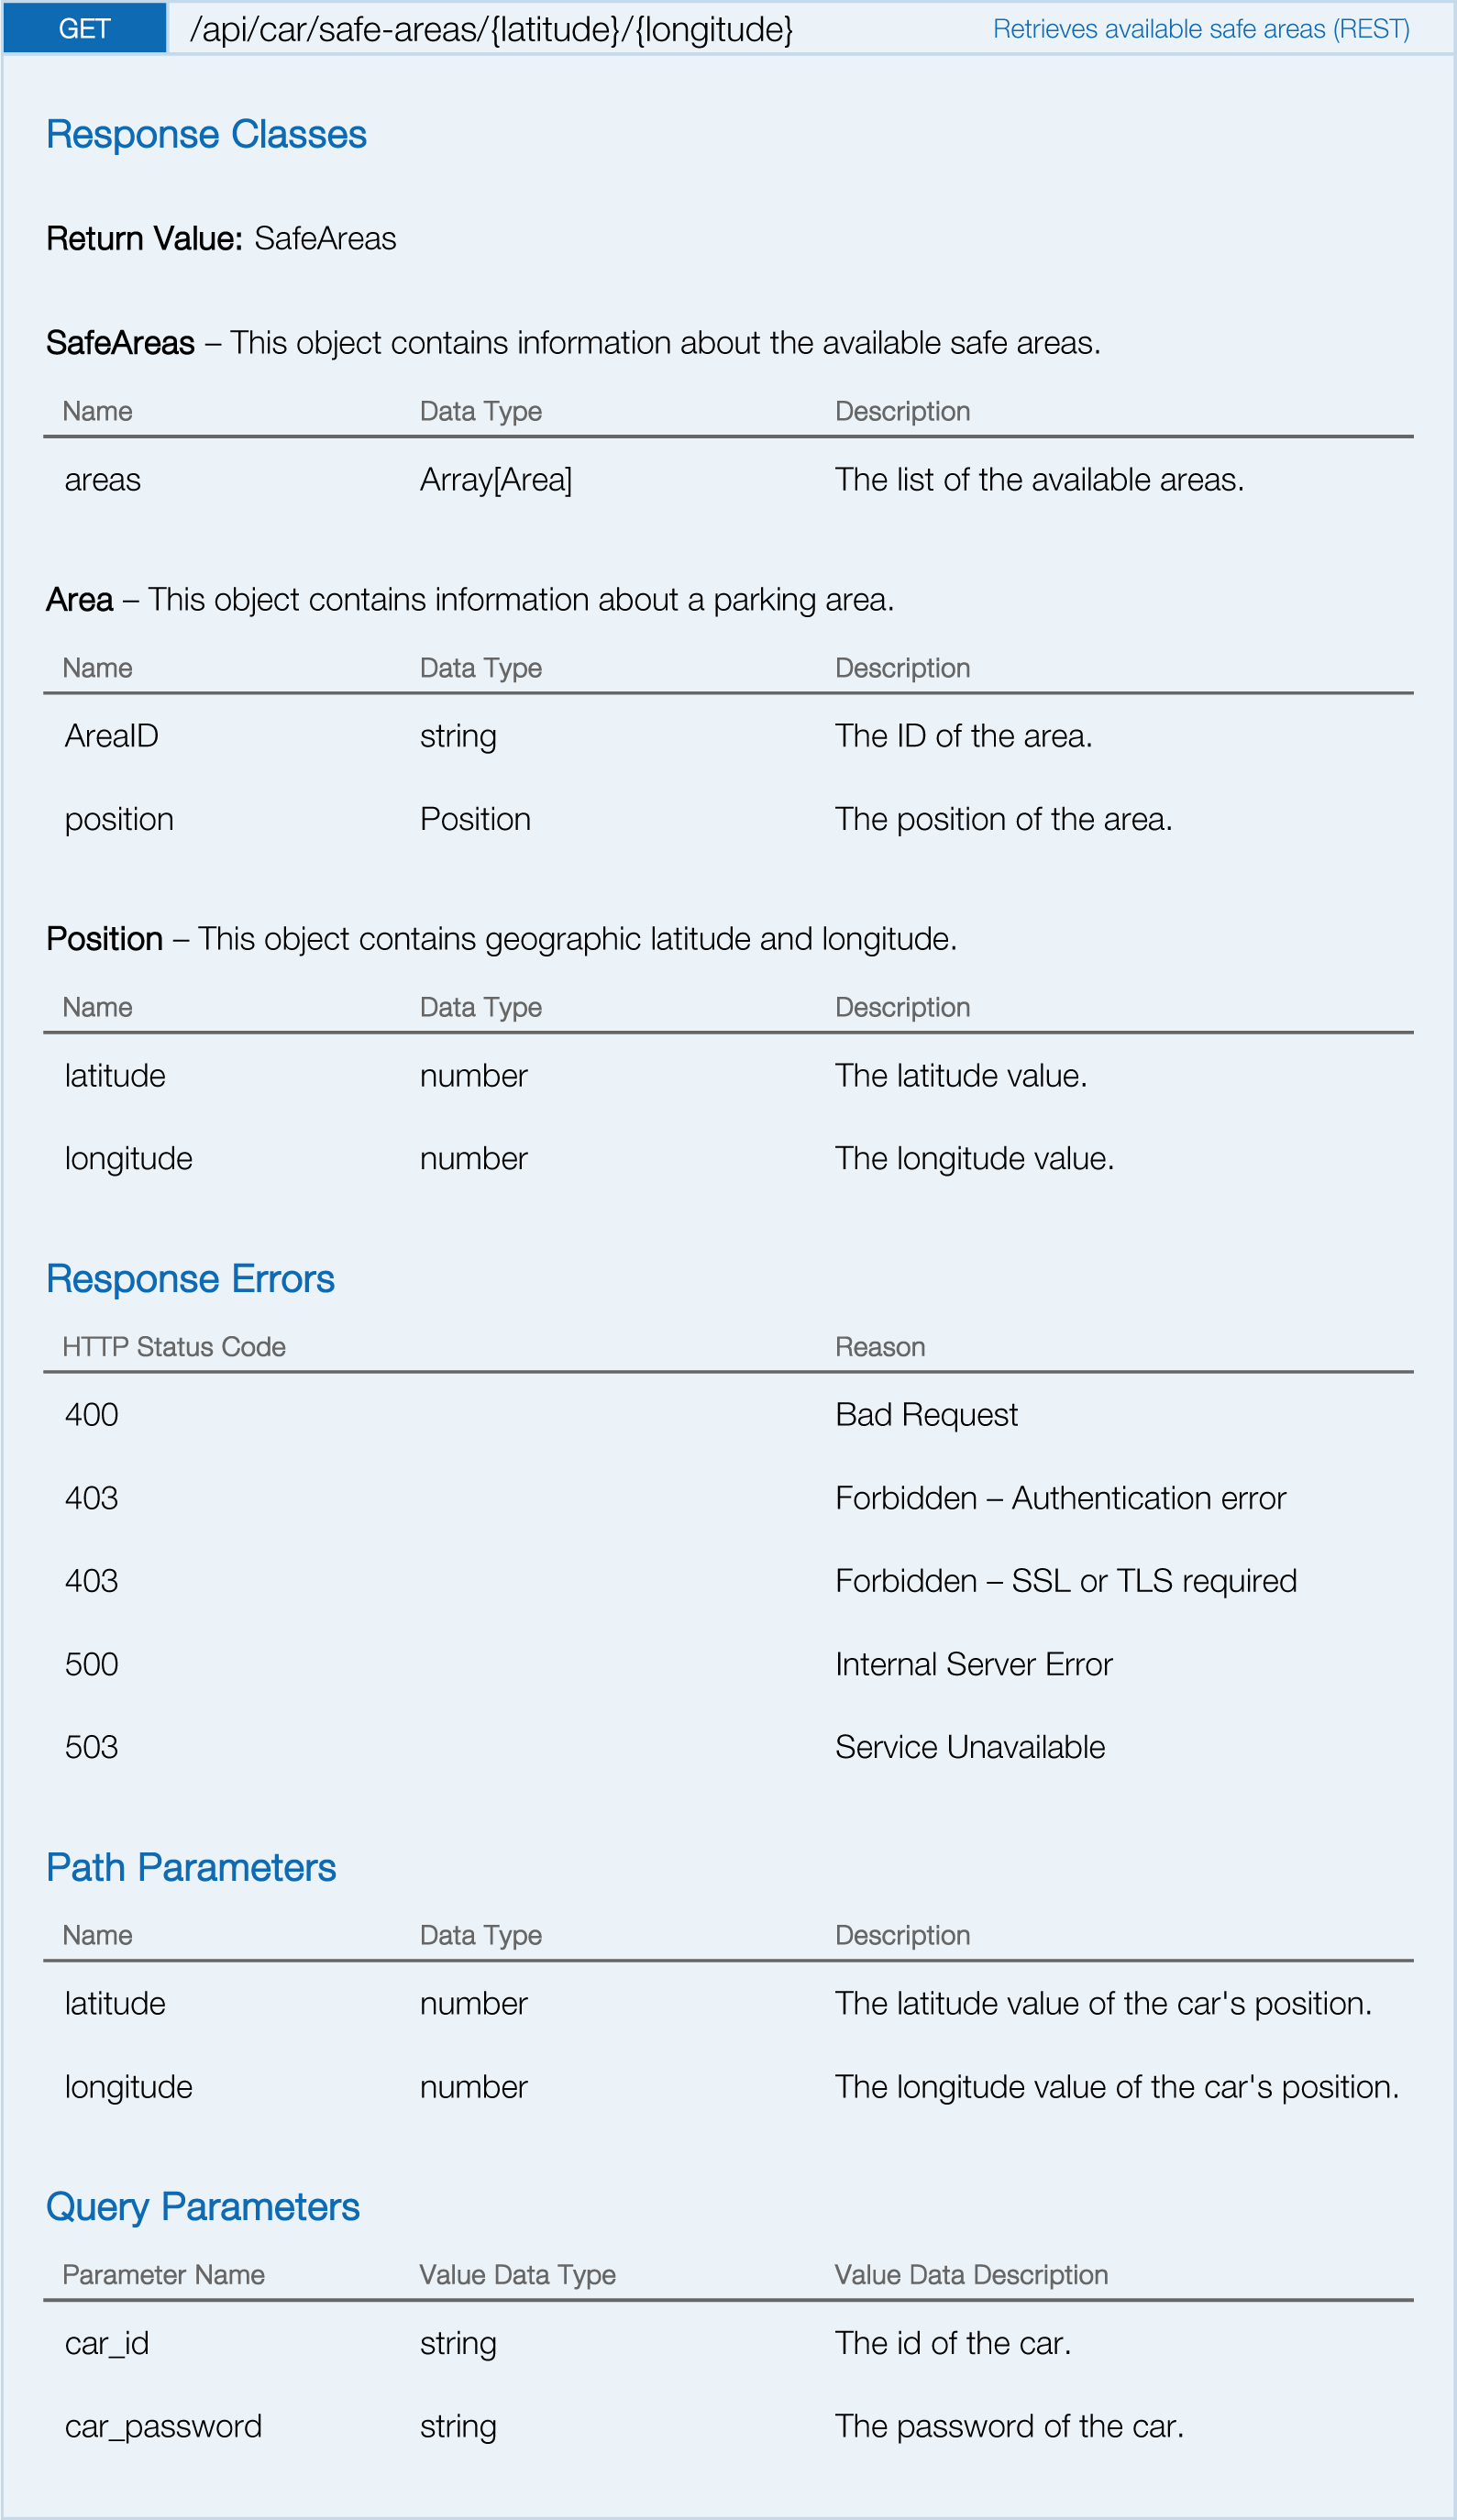
\includegraphics[height=550px, keepaspectratio]{apitables/APISafeAreas.png}
    	\label{fig:api-safe-areas}
\end{figure}

\subsubsubsection{Other requests}

There are other requests, but they are not relevant as the previous requests. For instance:

\begin{itemize}
	\item update user's information.
	\item execute payments.
	\item get the current charge of a rent.
	\item get information about a single car.
\end{itemize}
